%%%% ijcai25.tex

\typeout{IJCAI--25 Instructions for Authors}

% These are the instructions for authors for IJCAI-25.

\documentclass{article}
\pdfpagewidth=8.5in
\pdfpageheight=11in

% The file ijcai25.sty is a copy from ijcai22.sty
% The file ijcai22.sty is NOT the same as previous years'
\usepackage{ijcai25}

% Use the postscript times font!
\usepackage{times}
\usepackage{soul}
\usepackage{url}
\usepackage[hidelinks]{hyperref}
\usepackage[utf8]{inputenc}
\usepackage[small]{caption}
\usepackage{graphicx}
\usepackage{amsmath}
\usepackage{amsthm}
\usepackage{booktabs}
\usepackage{algorithm}
\usepackage{algorithmic}
%\usepackage[switch]{lineno}
%\usepackage[nonumberlist]{lineno}
\usepackage{multirow}
\usepackage[table,xcdraw]{xcolor}
\usepackage{tabularx}
\usepackage{amssymb}
\usepackage{makecell}

\usepackage{tikz}
\usepackage{hyperref}
\usetikzlibrary{shapes.geometric, arrows, mindmap}
\usetikzlibrary{positioning}  

%\bibliographystyle{unsrt} % 按引用顺序排列

% Comment out this line in the camera-ready submission
%\linenumbers

\urlstyle{same}

% the following package is optional:
%\usepackage{latexsym}

% See https://www.overleaf.com/learn/latex/theorems_and_proofs
% for a nice explanation of how to define new theorems, but keep
% in mind that the amsthm package is already included in this
% template and that you must *not* alter the styling.
\newtheorem{example}{Example}
\newtheorem{theorem}{Theorem}
\newtheorem{definition}{Definition}
\renewcommand{\thefootnote}{\fnsymbol{footnote}}

% Following comment is from ijcai97-submit.tex:
% The preparation of these files was supported by Schlumberger Palo Alto
% Research, AT\&T Bell Laboratories, and Morgan Kaufmann Publishers.
% Shirley Jowell, of Morgan Kaufmann Publishers, and Peter F.
% Patel-Schneider, of AT\&T Bell Laboratories collaborated on their
% preparation.

% These instructions can be modified and used in other conferences as long
% as credit to the authors and supporting agencies is retained, this notice
% is not changed, and further modification or reuse is not restricted.
% Neither Shirley Jowell nor Peter F. Patel-Schneider can be listed as
% contacts for providing assistance without their prior permission.

% To use for other conferences, change references to files and the
% conference appropriate and use other authors, contacts, publishers, and
% organizations.
% Also change the deadline and address for returning papers and the length and
% page charge instructions.
% Put where the files are available in the appropriate places.


% PDF Info Is REQUIRED.

% Please leave this \pdfinfo block untouched both for the submission and
% Camera Ready Copy. Do not include Title and Author information in the pdfinfo section
\pdfinfo{
/TemplateVersion (IJCAI.2025.0)
}

\title{Survey on Strategic Mining in Blockchain: A Reinforcement Learning Approach}
%Reinforcement Learning in Blockchain: A Survey of Its Use in Strategic Mining Behavior Analysis
%关于使用Reinforcement Learning分析区块链上策略挖矿行为的Survey。
% A Survey on the Application of Reinforcement Learning for Analyzing Strategic Mining Behavior on Blockchain
% A Survey of Reinforcement Learning Approaches for Strategy Mining Analysis in Blockchain

% Single author syntax
% \author{
%     Author Name
%     \affiliations
%     Affiliation
%     \emails
%     email@example.com
% }

% Multiple author syntax (remove the single-author syntax above and the \iffalse ... \fi here)
%\iffalse
\author{
Jichen Li$^{1,2\dagger}$\and
Lijia Xie$^{1\dagger}$\and
Hanting Huang$^{1,4}$\and
Bo Zhou$^1$\and
Binfeng Song$^{1,4}$\and \\
Wanying Zeng$^{1,3}$\and
Xiaotie Deng$^{1,2*}$\And
Xiao Zhang$^{1,3,5*}$\\
\affiliations
$^1$Zhongguancun Laboratory\\
$^2$Center on Frontiers of Computing
Studies, Computer Science Department, Peking University\\
$^3$LMIB and School of Mathematical Sciences, Beihang University\\
$^4$LMIB and Institute of Artificial Intelligence, Beihang University\\
$^5$Hangzhou International Innovation Institute of Beihang University\\
\emails
\{limo923, xiaotie\}@pku.edu.cn,
\{xielj, zhoubo\}@zgclab.edu.cn,\\
\{hantinghuang, zb2342110, zengzeng, xiao.zh\}@buaa.edu.cn
}

\begin{document}

\maketitle
\footnotetext{$^{\dagger}$Equal Contribution.}
\footnotetext{$^{*}$Corresponding Authors.}
\begin{abstract}
Strategic mining attacks, such as selfish mining, exploit blockchain consensus protocols by deviating from honest behavior to maximize rewards.
Markov Decision Process (MDP) analysis faces scalability challenges in modern digital economics, including blockchain.
To address these limitations, reinforcement learning (RL) provides a scalable alternative, enabling adaptive strategy optimization in complex dynamic environments.

In this survey, we examine RL's role in strategic mining analysis, comparing it to MDP-based approaches. We begin by reviewing foundational MDP models and their limitations, before exploring RL frameworks that can learn near-optimal strategies across various protocols.
Building on this analysis, we compare RL techniques and their effectiveness in deriving security thresholds, such as the minimum attacker power required for profitable attacks. 
Expanding the discussion further, we classify consensus protocols and propose open challenges, such as multi-agent dynamics and real-world validation.

This survey highlights the potential of reinforcement learning (RL) to address the challenges of selfish mining, including protocol design, threat detection, and security analysis, while offering a strategic roadmap for researchers in decentralized systems and AI-driven analytics.
\end{abstract}

% \section{Introduction}

Deep Reinforcement Learning (DRL) has emerged as a transformative paradigm for solving complex sequential decision-making problems. By enabling autonomous agents to interact with an environment, receive feedback in the form of rewards, and iteratively refine their policies, DRL has demonstrated remarkable success across a diverse range of domains including games (\eg Atari~\citep{mnih2013playing,kaiser2020model}, Go~\citep{silver2018general,silver2017mastering}, and StarCraft II~\citep{vinyals2019grandmaster,vinyals2017starcraft}), robotics~\citep{kalashnikov2018scalable}, communication networks~\citep{feriani2021single}, and finance~\citep{liu2024dynamic}. These successes underscore DRL's capability to surpass traditional rule-based systems, particularly in high-dimensional and dynamically evolving environments.

Despite these advances, a fundamental challenge remains: DRL agents typically rely on deep neural networks, which operate as black-box models, obscuring the rationale behind their decision-making processes. This opacity poses significant barriers to adoption in safety-critical and high-stakes applications, where interpretability is crucial for trust, compliance, and debugging. The lack of transparency in DRL can lead to unreliable decision-making, rendering it unsuitable for domains where explainability is a prerequisite, such as healthcare, autonomous driving, and financial risk assessment.

To address these concerns, the field of Explainable Deep Reinforcement Learning (XRL) has emerged, aiming to develop techniques that enhance the interpretability of DRL policies. XRL seeks to provide insights into an agent’s decision-making process, enabling researchers, practitioners, and end-users to understand, validate, and refine learned policies. By facilitating greater transparency, XRL contributes to the development of safer, more robust, and ethically aligned AI systems.

Furthermore, the increasing integration of Reinforcement Learning (RL) with Large Language Models (LLMs) has placed RL at the forefront of natural language processing (NLP) advancements. Methods such as Reinforcement Learning from Human Feedback (RLHF)~\citep{bai2022training,ouyang2022training} have become essential for aligning LLM outputs with human preferences and ethical guidelines. By treating language generation as a sequential decision-making process, RL-based fine-tuning enables LLMs to optimize for attributes such as factual accuracy, coherence, and user satisfaction, surpassing conventional supervised learning techniques. However, the application of RL in LLM alignment further amplifies the explainability challenge, as the complex interactions between RL updates and neural representations remain poorly understood.

This survey provides a systematic review of explainability methods in DRL, with a particular focus on their integration with LLMs and human-in-the-loop systems. We first introduce fundamental RL concepts and highlight key advances in DRL. We then categorize and analyze existing explanation techniques, encompassing feature-level, state-level, dataset-level, and model-level approaches. Additionally, we discuss methods for evaluating XRL techniques, considering both qualitative and quantitative assessment criteria. Finally, we explore real-world applications of XRL, including policy refinement, adversarial attack mitigation, and emerging challenges in ensuring interpretability in modern AI systems. Through this survey, we aim to provide a comprehensive perspective on the current state of XRL and outline future research directions to advance the development of interpretable and trustworthy DRL models.
% \section{Consensus and Strategic Mining}
% intro里面的一些拿过来?

\subsection{SM MDP}

Formally, if all other participants are following the standard protocol, the attacker faces a single-player decision problem of the form $M := <S, A, P, R>$, where $S$ is the state space, $A$ the action space, $P$ a stochastic transition matrix that describes the probability of transitioning between states, and $R$ the reward matrix. Though similar in structure, we do not regard $M$ as an MDP, since the objective function is nonlinear: The player aims to maximize its share of the accepted blocks, rather than the absolute number of its own accepted ones; its goal is to have a greater return-on-investment than its counterparts

\textbf{Action space}
Actions. We begin with the description of the action space A, which will motivate the nontrivial construction of the state space.
\begin{itemize}
    \item Adopt. The action \emph{adopt} is always feasible, and represents the attacker’s acceptance of the honest network’s chain. The $a$ blocks in the attacker’s current chain are discarded.
    \item Override. The action \emph{override} represents the publication of the attacker’s blocks, and is feasible whenever $a > h$.
    \item Match. This action represents the case where the most recent block was built by the honest network, and the attacker now publishes a conflicting block of the same height. This action is not always feasible (the attacker must have a block prepared in advance to execute such a race). The statespace explicitly encodes the feasibility status of this action (see below).
    \item Wait. Lastly, the wait action, which is always feasible, implies that the attacker does not publish new blocks, but keeps working on its branch until a new block is built.
\end{itemize}

\textbf{State space}
The state space, denoted $S$, is defined by 3-tuples of the form $(a, h, fork)$. The first two entries represent the lengths of the attacker’s chain and the honest network’s chain, built after the latest fork (that is, above the most recent block accepted by all). The field fork obtains three values, dubbed irrelevant, relevant and active. State of the form $(a, h, relevant)$ means that the previous state was of the form $(a, h - 1, \cdot)$; this implies that if $a \geq h$, match is feasible. Conversely, $(a, h, irrelevant)$ denotes the case where the previous state was $(a - 1, h, \cdot)$, rendering match now ineffective, as all honest nodes received already the $h$’th block. The third label, active, represents the case where the honest network is already split, due to a previous match action; this information affects the transition to the next state, as described below. We will refer to states as $(a, h)$ or $(a, h, \cdot)$, in contexts where the fork label plays no effective role.

\textbf{Reward}
In order to keep the time averaging of rewards in scale, every state transition corresponds to the creation of a new block. The initial state $X_0$ is $(1, 0, irrelevant)$ w.p. $\alpha$ or $(0, 1, irrelevant)$ w.p. $(1 - \alpha)$. Rewards are given as elements in $N^2$, where the first entry represents blocks of the attacker that have been accepted by all parties, and the second one, similarly, for those of the honest network.

The transition matrix $P$ and reward matrix $R$ are succinctly described in Table. Largely, an adopt action “resets” the game, hence the state following
it has the same distribution as $X_0$; its immediate reward is $h$ in the  coordinate corresponding to the honest network. An override reduces the attacker’s secret chain by $h+1$ blocks, which it publishes, and which the honest network accepts. This bestows a reward of $h + 1$ blocks to the attacker. The state following a match action depends on whether the next block is created by the attacker $(\alpha)$, by honest nodes working on their branch of the chain $((1 - \gamma) \cdot (1 - \alpha))$, or by an honest node which accepted the sub-chain that the attacker published $(\gamma \cdot (1-\alpha))$. In the latter case, the attacker has effectively overridden the honest network’s previous chain, and is awarded $h$ accordingly.

\begin{table}[h]
\label{Table1}
\centering
\begin{tabular}{|l|l|l|l|}
\hline
\textbf{State × Action}                    & \textbf{State}                    & \textbf{Probability}          & \textbf{Reward}  \\ \hline
$(a,h,\cdot), \text{adopt}$                & $(1,0,\text{irrelevant})$         & $\alpha$                      & $(0,h)$          \\ \cline{2-4} 
                                           & $(0,1,\text{irrelevant})$         & $1-\alpha$                    & $(0,h)$          \\ \hline
$(a,h,\cdot), \text{override}^\dagger$     & $(a-h,0,\text{irrelevant})$       & $\alpha$                      & $(h+1,0)$        \\ \cline{2-4} 
                                           & $(a-h-1,1,\text{relevant})$       & $1-\alpha$                    & $(h+1,0)$        \\ \hline
$(a,h,\text{irrelevant}), \text{wait}$     & $(a+1,h,\text{irrelevant})$       & $\alpha$                      & $(0,0)$          \\ \hline
$(a,h,\text{relevant}), \text{wait}$       & $(a,h+1,\text{relevant})$         & $1-\alpha$                    & $(0,0)$          \\ \hline
$(a,h,\text{active}), \text{wait}$         & $(a+1,h,\text{active})$           & $(\gamma) \cdot (1-\alpha)$   & $(0,0)$          \\ \hline
$(a,h,\text{relevant}), \text{match}^\ddagger$ & $(a-h,1,\text{relevant})$        & $\gamma \cdot (1-\alpha)$     & $(h,0)$          \\ \cline{2-4} 
                                           & $(a,h+1,\text{relevant})$         & $(1-\gamma) \cdot (1-\alpha)$ & $(0,0)$          \\ \hline
\end{tabular}
\caption{A description of the transition and reward matrices $P$ and $R$ in the decision problem $M$. The third column contains the probability of transiting from the state specified in the left-most column, under the action specified therein, to the state on the second one. The corresponding two-dimensional reward (the reward of the attacker and that of the honest nodes) is specified on the right-most column.}
\footnotesize{$^\dagger$feasible only when $a \geq h$}
\footnotesize{$^\ddagger$feasible only when $a \geq h$}
\end{table}

\textbf{Objective Function}
As explained in the introduction, the attacker aims to maximize its relative revenue, rather than its absolute one as usual in MDPs. Let $\pi$ be a policy of the player; we will write $\pi(a, h, fork)$ for the action that $\pi$ dictates be taken at state $(a, h, fork)$. Denote by $X^{\pi}_t$ the state visited by time $t$ under $\pi$, and let $r(x, y, \pi) = (r1(x, y, \pi), r2(x, y, \pi))$ be the immediate reward from transiting from state x to state y, under the action dictated by $\pi$. $X^{\pi}_t$ will denote the $t$’th state that was visited. We will abbreviate $r_t(X^\pi_t ,X^\pi_{t+1}, \pi)$ and write simply $r_t(\pi)$ or even $r_t$, when context is clear. The objective function of the player is its relative payoff, defined by
\begin{align}
    REV := \mathcal{E} \left[ \liminf_{T \rightarrow \infty} \frac{\sum_{t=1}^T r_t^1(\pi)}{\sum_{t=1}^T(r_t^1(\pi)+r_t^2(\pi))} \right]    
\end{align}
We will specify the parameters of REV depending on the context (e.g.,
$REV(\pi, \alpha, \gamma), REV(\pi), REV(\alpha))$, and will occasionally denote the value of $REV$ by $\rho$. In addition, for full definiteness of $REV$, we rule out pathological behaviours in which the attacker waits forever—formally, the expected time for the next non-null action of the attacker must be finite.
% \section{Methodology}

\subsection{Markov Reward Process}

A Markov chain is a stochastic process that evolves through a sequence of states, where the probability of transitioning to the next state depends only on the current state (i.e., it has memoryless property). A Markov chain is defined by a finite or countably infinite set of states, transition probabilities between states, and an initial probability distribution over the states. 

\begin{definition}
    A Markov chain is a stochastic process $(X_t)_{t=0}^{\infty}$ with the following:
    \begin{itemize}
        \item A countable or finite state space $\{s_0, s_1, ... ,s_n\} \in S$.
        \item A transition matrix $P = (p_{ij})$, where $p_{ij}$ represents the probability of transitioning from state $s_i$ to state $s_j$.
        \item Markov property:
        $P(X_{N+1} = s_i | X_0 = s_{t_0}, X_1 = s_{t_1}, \ldots, X_{N} = s_{t_N}) = P(X_{N+1} = s_i | X_N = s_{t_N})$
    \end{itemize}
\end{definition}

%Markov chains 在区块链共识建模中有广泛的应用。 

\subsection{Reinforcement Learning}

Reinforcement learning is a class of machine learning algorithms that enables an agent to learn to make decisions or take actions in an environment to maximize a cumulative reward.
The agent learns through trial and error, receiving feedback from the environment through rewards or punishments.
Deep reinforcement learning combines reinforcement learning with deep learning techniques, using neural networks to approximate the value function or policy of the agent.
It is a suitable method to solve complex Markov Reward Process problems in which the environment responds reward to the agent's actions according to the transition probability.

There has been growing interest in applying reinforcement learning techniques, including deep reinforcement learning, to blockchain research in recent years.
%Paper description

\subsection{Security Threshold}

%define of Security Threshold


\subsection{MDP Model}
Formally, if all other participants are following the standard protocol, the attacker faces a single-player decision problem of the form $M := <S, A, P, R>$, where $S$ is the state space, $A$ the action space, $P$ a stochastic transition matrix that describes the probability of transitioning between states, and $R$ the reward matrix. Though similar in structure, we do not regard $M$ as an MDP, since the objective function is nonlinear: The player aims to maximize its share of the accepted blocks, rather than the absolute number of its own accepted ones; its goal is to have a greater return-on-investment than its counterparts

\textbf{Action space}
Actions. We begin with the description of the action space A, which will motivate the nontrivial construction of the state space.
\begin{itemize}
    \item Adopt. The action \emph{adopt} is always feasible, and represents the attacker’s acceptance of the honest network’s chain. The $a$ blocks in the attacker’s current chain are discarded.
    \item Override. The action \emph{override} represents the publication of the attacker’s blocks, and is feasible whenever $a > h$.
    \item Match. This action represents the case where the most recent block was built by the honest network, and the attacker now publishes a conflicting block of the same height. This action is not always feasible (the attacker must have a block prepared in advance to execute such a race). The statespace explicitly encodes the feasibility status of this action (see below).
    \item Wait. Lastly, the wait action, which is always feasible, implies that the attacker does not publish new blocks, but keeps working on its branch until a new block is built.
\end{itemize}

\textbf{State space}
The state space, denoted $S$, is defined by 3-tuples of the form $(a, h, fork)$. The first two entries represent the lengths of the attacker’s chain and the honest network’s chain, built after the latest fork (that is, above the most recent block accepted by all). The field fork obtains three values, dubbed irrelevant, relevant and active. State of the form $(a, h, relevant)$ means that the previous state was of the form $(a, h - 1, \cdot)$; this implies that if $a \geq h$, match is feasible. Conversely, $(a, h, irrelevant)$ denotes the case where the previous state was $(a - 1, h, \cdot)$, rendering match now ineffective, as all honest nodes received already the $h$’th block. The third label, active, represents the case where the honest network is already split, due to a previous match action; this information affects the transition to the next state, as described below. We will refer to states as $(a, h)$ or $(a, h, \cdot)$, in contexts where the fork label plays no effective role.

\textbf{Reward}
In order to keep the time averaging of rewards in scale, every state transition corresponds to the creation of a new block. The initial state $X_0$ is $(1, 0, irrelevant)$ w.p. $\alpha$ or $(0, 1, irrelevant)$ w.p. $(1 - \alpha)$. Rewards are given as elements in $N^2$, where the first entry represents blocks of the attacker that have been accepted by all parties, and the second one, similarly, for those of the honest network.

The transition matrix $P$ and reward matrix $R$ are succinctly described in Table. Largely, an adopt action “resets” the game, hence the state following
it has the same distribution as $X_0$; its immediate reward is $h$ in the  coordinate corresponding to the honest network. An override reduces the attacker’s secret chain by $h+1$ blocks, which it publishes, and which the honest network accepts. This bestows a reward of $h + 1$ blocks to the attacker. The state following a match action depends on whether the next block is created by the attacker $(\alpha)$, by honest nodes working on their branch of the chain $((1 - \gamma) \cdot (1 - \alpha))$, or by an honest node which accepted the sub-chain that the attacker published $(\gamma \cdot (1-\alpha))$. In the latter case, the attacker has effectively overridden the honest network’s previous chain, and is awarded $h$ accordingly.

\textbf{Objective Function}
As explained in the introduction, the attacker aims to maximize its relative revenue, rather than its absolute one as usual in MDPs. Let $\pi$ be a policy of the player; we will write $\pi(a, h, fork)$ for the action that $\pi$ dictates be taken at state $(a, h, fork)$. Denote by $X^{\pi}_t$ the state visited by time $t$ under $\pi$, and let $r(x, y, \pi) = (r1(x, y, \pi), r2(x, y, \pi))$ be the immediate reward from transiting from state x to state y, under the action dictated by $\pi$. $X^{\pi}_t$ will denote the $t$’th state that was visited. We will abbreviate $r_t(X^\pi_t ,X^\pi_{t+1}, \pi)$ and write simply $r_t(\pi)$ or even $r_t$, when context is clear. The objective function of the player is its relative payoff, defined by
$$
    REV := \mathcal{E} \left[ \liminf_{T \rightarrow \infty} \frac{\sum_{t=1}^T r_t^1(\pi)}{\sum_{t=1}^T(r_t^1(\pi)+r_t^2(\pi))} \right]    
$$
We will specify the parameters of REV depending on the context (e.g.,
$REV(\pi, \alpha, \gamma), REV(\pi), REV(\alpha))$, and will occasionally denote the value of $REV$ by $\rho$. In addition, for full definiteness of $REV$, we rule out pathological behaviours in which the attacker waits forever—formally, the expected time for the next non-null action of the attacker must be finite.
% \section{Results}

% 1.在基础Consensus基础上,考虑了哪些特殊的环境设计
% 2.Selfish(Strategic) miner strategy space
% 3.Honest(Other) miner's action
% 4.MDP/Learning Solving Methods or Technique
% 5.Results: security threshold, some insight to explain it.



%\begin{table*}[ht]
%\centering
%\caption{Consensus Mechanism Classification}
%\renewcommand{\arraystretch}{1.5} % Adjust row height
%\setlength{\tabcolsep}{5pt} % Adjust column spacing
%\begin{tabular}{|p{3cm}|p{3cm}|p{5cm}|p{6cm}|}
%\hline
%\multicolumn{2}{|c|}{\textbf{Category}} & \multicolumn{1}{c|}{\textbf{Consensus Protocols}} & \multicolumn{1}{c|}{\textbf{Description}} \\ \hline
\multicolumn{1}{|c|}{}                                    & Longest Chain Rule  & Bitcoin\cite{nakamoto2008bitcoin}, Ethereum 1.0\cite{wood2014ethereum}, FruitChain\cite{pass2017fruitchains}                        & Based on PoW, selecting the longest chain by computational work. \\ \cline{2-4}
\multicolumn{1}{|c|}{\multirow{-2}{*}{Chain-based Rules}} & Heaviest Chain Rule & Ouroboros\cite{kiayias2017ouroboros}, PoST \cite{moran2019simple} & Based on PoS or storage, selecting the chain with the highest accumulated weight. \\ \hline
\multicolumn{2}{|c|}{Vote-based Rules}                                          & PBFT\cite{castro1999practical}, Tendermint \cite{buchman2016tendermint}, Diem BFT \cite{team2021diembft}, HotStuff\cite{yin2019hotstuff}, Ethereum 2.0\cite{buterin2020combining} & Deterministic consensus with a voting mechanism, ensuring finality without forks and randomness. \\ \hline
\multicolumn{2}{|c|}{Parallel Confirmation Rules}                                           & Avalanche \cite{rocket2019scalable}, Sui \cite{blackshear2023sui} & Probabilistic consensus based on DAG, supporting high throughput and scalability. \\ \hline
\end{tabular}
\end{table*}


\subsection{Proof of Work Consensus}

\textbf{Selfish mining} - Jichen Li
It has long been believed that the Bitcoin protocol is incentive-compatible. However, Eyal and Sirer~\cite{eyal2014majority} indicate this is not the case. It describes a well-known attack called selfish mining. A pool could receive higher rewards than its fair share via the selfish mining strategy. This attack ingeniously exploits the conflict-resolution rule of the Bitcoin protocol, in which when encountering a fork, only one chain of blocks will be considered valid. With the selfish mining strategy, the attacker deliberately creates a fork and forces honest miners to waste efforts on a stale branch. Specifically, the selfish pool strategically keeps its newly found block secret rather than publishing it immediately. Afterward, it continues to mine on the head of this private branch. When the honest miners generate a new block, the selfish pool will correspondingly publish one private block at the same height and thus create a fork. Once the selfish pool's leads are reduced to two, an honest block will prompt it to reveal all its private blocks. As a well-known conclusion, assuming that the honest miners apply the uniform tie-breaking rule, if the fraction of the selfish pool's mining power is greater than $25\%$, it will always get more benefit than behaving honestly.

\textbf{Optimal Selfish mining} - Jichen Li
\cite{sapirshtein2016optimal} extend the underlying model for selfish mining attacks, and provide an algorithm to find Q-optimal policies for attackers within the model, as well as tight upper bounds on the revenue of optimal policies. 
As a consequence, the algorithm are able to provide lower bounds on the computational power an attacker needs in order to benefit from selfish mining. 
Paper find that the profit threshold – the minimal fraction of resources required for a profitable attack – is strictly lower than the one induced by the \cite{eyal2014majority} scheme. Indeed, the policies given by our algorithm dominate orginal selfish mining strategy, by better regulating attack-withdrawals.

\textbf{A Better Method to Analyze Blockchain Consistency} - Jichen Li
When considering how to analyze a PoW blockchain protocol, the formal frameworks only analyze the consistency and liveness of the chain.
Paper \cite{kiffer2018better} provides a Markov-chain based method for analyzing the consistency properties of blockchain protocols.
They consider a partially synchronous network that proposed blocks in the rounds and an adaptive corrupt adversary.
The adversary can break blockchain consistency by processing a family of delaying attacks, in which they will withhold their block and broadcast it when any honest miner finds a block.
By analyzing this attack, the authors show strong concentration bounds to demonstrate how long a participant should wait before considering a high-value transaction to be confirmed.

\textbf{Lay Down the Common Metrics: Evaluating Proof-of-Work Consensus Protocols’ Security} - Binfeng Song, Lijia Xie
\cite{zhang2019lay} employed a multi-metric evaluation framework based on Markov decision processes to quantitatively assess the chain quality and attack resistance of several existing enhanced PoW protocols. In this framework, the metric of incentive compatibility serves as an indicator of a protocol's resistance to selfish mining.
In the analysis of selfish mining strategies using MDP modeling, 
selfish miners can secretly withhold their discovered blocks, revealing their chain only when it surpasses the length of the public chain or when their lead is reduced to a single block. Conversely, honest miners adheres to protocol rules, promptly publishing blocks and choosing the longest chain for mining. The conclusions suggest that current enhanced PoW protocols fail to achieve optimal chain quality or robust attack resistance. This shortfall is attributed to the inherent dilemma in existing protocols between rewarding malicious actions and penalizing adherence to the protocol.

\textbf{SquirRL} - Wanying Zeng, Bo Zhou
\cite{hou2019squirrl} introduce SquirRL, a framework that leverages deep reinforcement learning to explore vulnerabilities in blockchain incentive mechanisms and recover adversarial strategies. Application of SquirRL successfully uncovers previously known attacks, including the optimal selfish mining attack in Bitcoin \cite{sapirshtein2016optimal}, and the Nash equilibrium in block withholding attacks\cite{eyal2015miner}. 

SquirRL applies to selfish-mining evaluation in blockchain consensus/incentive protocols through the following steps:
(a)Environment Construction: The environment involves features and action spaces reflecting the views and capabilities of participating agents. SquirRL considers different environment designs, including single selfish miner, and multiple selfish miners, as well as dynamic and stochastic environment designs, on top of the basic consensus protocol.
(b)Adversarial Model Selection: The protocol designer selects an adversarial model, including the numbers and types of agents, to explore various adversarial strategies.
(c)RL Algorithm Selection: The protocol designer selects an RL algorithm appropriate for the environment and adversarial model, associating it with a reward function and hyperparameters. SquirRL utilizes deep reinforcement learning (DRL) algorithms to solve Markov Decision Processes (MDPs), including both value-based methods and policy gradient methods.
(d)Training and Evaluation: SquirRL trains DRL agents in the selected environment and evaluates the performance of various strategies, including selfish mining, against baseline strategies and known theoretical results.

The paper yields novel empirical insights. Firstly, a counterintuitive flaw is identified in the widely used rushing adversary model when applied to multi-agent Markov games with incomplete information.
Secondly, contrary to previous assumptions, the optimal selfish mining strategy identified in \cite{sapirshtein2016optimal} is not a Nash equilibrium in the multi-agent selfish mining context. The results suggest (though not conclusively proven) that when more than two competing agents engage in selfish mining, no profitable Nash equilibrium exists. This observation aligns with the lack of observed selfish mining behavior in real-world scenarios.
Thirdly, a novel attack is uncovered on a simplified version of Ethereum’s finalization mechanism, Casper the Friendly Finality Gadget (FFG). This attack allows a strategic agent to amplify her rewards by up to 30\%.


\textbf{WeRLman} - Hanting Huang, Nuojing Liang
Incentives are crucial to ensuring the security of proof-of-work blockchain protocols. In the operation of blockchain systems, whale transactions, characterized by offering additional transaction costs, occur occasionally. WeRLman is the first selfish-mining analysis model considering both subsidy and transaction fees\cite{bar2022werlman}. Like Squirl, WeRLman describes blockchain through a Markov Decision Process (MDP). To cope with the complexity of the model and the large policy space, WeRLman utilizes a deep reinforcement learning framework inspired by the principles of AlphaGo Zero and incorporates Monte Carlo Tree Search (MCTS) and Deep Q Network (DQN) methods. Through experiments extracted from the Bitcoin platform data, analysis based on WeRLman reveals a clear inverse relationship between fee changes and the system security threshold. It is worth noting that the security threshold is considerably lower in the case of whale transactions compared to the security threshold of 0.25 analyzed by the previous model built under constant rewards. Specifically, based on Bitcoin's historical fees with its minting strategy, the deviation thresholds would be reduced to 0.2 in 10 years, 0.17 in 20 years, and 0.12 in 30 years. Based on the current transaction costs of the Ethernet smart contract platform, the security threshold would be reduced to 0.17, which is below the common sizes of large miners.

\textbf{Deep Bribe: Predicting the Rise of Bribery in Blockc-hain Mining with Deep RL} - Jiawei Nie, Feifan Wang 
\cite{bar2023deep}Building upon WeRLman, the article further considers the impact of petty compliant miners on the security threshold. Specifically, as transaction fees relative to the block's inherent reward (BTC) gradually increase, some miners tend to favor chains with more transaction fees when producing forks, leading to the emergence of undercutting attacks. In this environment, selfish miners can attract petty compliant miners to mine on their forked chain by creating equally long chains with lower transaction fees, resulting in a lower security threshold. For the MDP Solving Method, PTO is first used for MDP transformation, followed by WeRLman for solving (based on MCTS and DQN). In the model of this article, when the proportion of petty compliant miners $\beta\geq$  0.75, the obtained security thresholds are respectively below 0.19 (additional transaction fee F = 0.14) and 0.13 (F = 0.74). This reflects that when considering the MEV represented by transaction fee differences, undercutting attacks (or bribery) can exacerbate the threat of selfish mining.

\textbf{Insightful Mining} - Jichen Li
In this paper, first, we propose a novel strategy called insightful mining to counteract the selfish mining attack. 
By infiltrating an undercover miner into the selfish pool, the insightful pool could acquire the number of its hidden blocks.
We prove that, with this extra insight, the utility of the insightful pool is strictly greater than the selfish pool’s when they have the same mining power. 
Then we investigate the mining game where all pools can choose to be honest or take the insightful mining strategy. 
We characterize the Nash equilibrium of such a game and derive three corollaries: 
(a) each mining game has a pure Nash equilibrium; 
(b) there are at most two insightful pools under some equilibrium no matter how the mining power is distributed; 
(c) honest mining is a Nash equilibrium if the largest mining pool has a fraction of mining power no more than 1/3.
Our work explores, for the first time, the idea of spying in the selfish mining attack, which might shed new light on researchers in the field.

\textbf{Undetectable Selfish Mining} - Feifan Wang, Jichen Li
\cite{bahrani2023undetectable}This paper builds upon the selfish mining model proposed by Eyal and Sirer\cite{eyal2014majority}, introducing the concept of statistically detectable actions and designing selfish mining strategies that achieve statistical undetectability. Firstly, the paper extends the Nakamoto Consensus Game (NCG) to l-NCG by introducing a delay parameter, innovatively characterizing the natural occurrence rate and statistical distribution of orphan blocks using this delay parameter. Subsequently, the paper demonstrates that two classical selfish mining strategies—Selfish Mining and Strong Selfish Mining—are statistically detectable due to the presence of strategic players, which leads to non-independent and non-identically distributed probabilities of generating orphan blocks at different heights. Then, starting from Selfish Mining and Strong Selfish Mining, it achieves undetectability by modifying the block publication method while ensuring strict profitability. Specifically, strategic players devise appropriate Labeling Strategy and Broadcasting Strategy based on the state of the previous height, ensuring that the probability of generating orphan blocks at the next height remains constant at a specified value. Through simple mathematical derivation and exact MDP solutions verification, the paper indicates that when the hash rate of strategic players exceeds 0.382, suitable strategies can always be found to achieve additional profits in the sense of statistical undetectability.


\subsection{Proof of Stake Consensus}
\textbf{Deep Selfish Proposing in Longest-Chain Proof-of-Stake Protocols} - Hanting Huang, Qingmao Yao

Though the longest chain rule was originally designed for features of the proof-of-work (PoW) protocol, some PoS-based blockchain protocols have also adopted it as their consensus protocol. However, there is no mining process in PoS; instead, there is the election of proposers. The selfish mining attack is one of the most important threats that can undermine the longest-chain blockchain protocol. Not only PoW-based blockchains but also POS-based blockchains using the longest chain paradigm face the threat of selfish mining. Since POS-based blockchains do not involve a mining process, the term "selfish proposing" is used instead of selfish mining to describe this attack. Compared to PoW protocols, generating valid blocks in LC-PoS is effortless. Based on the phenomenon called nothing-at-stake, attackers can expand their attacking strategies and generate new attack actions. Also, PoS protocols suffer from a degree of predictability for the lottery mechanism that specifies the block proposer(s) for each slot. This work \cite{sarenche2024deep} considers the selfish proposing attack in the longest-chain PoS (LC-PoS) blockchains. By generalizing the nothing-at-stake selfish proposing attack with different levels of predictability, it is concluded that the proposing block ratio will be slightly increased with the Nothing-at-Stake phenomenon, and proposer predictability will considerably increase the attack block ratio. To analyze the selfish proposing attack in more complicated scenarios, this work uses a Deep Q-learning tool to analyze the selfish proposing attack and obtain the near-optimal attack strategy with varying stake shares.

\textbf{Formal Barriers to Longest-Chain Proof-of-Stake Protocols} - Lijia Xie, Binfeng Song

In the study by \cite{brown2019formal}, a model for PoS (Proof of Stake) cryptocurrencies was proposed to analyze security issues driven by incentives. The paper establishes two key properties: predictability and recency, ensuring that every protocol within the model satisfies at least one of these properties. Moreover, the security implications of predictability and recency indicate that every protocol is vulnerable to at least one type of attack, including selfish mining, double spending, or Nothing-at-Stake attacks. In contrast to the adversarial corruption found in PoW (Proof of Work) systems, the main findings of this paper highlight the formal barriers to designing incentive-compatible PoS cryptocurrencies, stemming from the inherent pseudorandomness of PoS systems.

\textbf{Optimal Strategic Mining Against Cryptographic Self-Selection in Proof-of-stake} - Bo Zhou, Wanying Zeng

The paper \cite{ferreira2022optimal} considers an adversary who aims to lead and win in the PoS election protocol, maximizing the number of rounds they can win, and indicates that the presence of an adversary can gain more benefits through strategy, regardless of the proportion of stacks they control. In the Cryptographic self-selection protocol, a leader needs to be elected for each round to generate blocks, and the election of the leader is related to the stakes held by the players and the seeds of current round of. The leader can generate biased seeds to make them advantageous in subsequent rounds of elections. Ferreira et al. showed that when the stack ratio mastered by strategy players is less than 0.38, they can win at most one round. They also proposed a 1-Lookahead strategy that can strictly outperform any honest strategy under any stack ratio. Finally, they proposed an algorithm to find the optimal strategy through MDP.

\section{Conclusion and Discussion}


% \section{Conclusion}

We justify that a flow matching generative model can produce dense and reliable rewards for training LLMs to explain the decisions of RL agents and other LLMs. 
Looking into the future, we envision extending this method to a general LLM training approach, automatically generating high-quality dense rewards, and ultimately reducing the reliance on human feedback. 

% Our method has the potential to facilitate human-AI collaboration applications, such as transportation, education, and security defense.

\newpage
\section{Impact Statements}
This paper presents work whose goal is to advance the field of machine learning by developing a model-agnostic explanation generator for intelligent agents, enhancing transparency and interpretability in agent decision prediction. The ability to generate effective and interpretable explanations has the potential to foster trust in AI systems, improving effectiveness in high-stakes applications such as healthcare, finance, and autonomous systems. Overall, we believe our work contributes positively to the broader AI ecosystem by promoting more explainable and trustworthy AI.

% 按新逻辑写的部分,上面先保留作参考
\section{Introduction}
\label{sec:intro}
In recent years, blockchain technology has been widely applied to solve problems in various domains, developing innovative solutions previously considered impossible.  
It all began with an inventive ledger design to record all transactions generated in a decentralized system called Bitcoin, invented by \cite{nakamoto2008bitcoin}.  
This revolutionary ledger design maintains a sequentially growing list of blocks, each containing several transactions and linked to the preceding block using cryptographic techniques.  
The process of adding new blocks is governed by a consensus mechanism called Proof of Work (PoW), in which participants, called miners, use their computational power to calculate a hash function.
The miner who finds a valid solution for this hash function can have the right to produce a new block and earn rewards for generating it.  
In the design of the Bitcoin protocol, each miner is expected to broadcast the generated block to the network immediately.  
As long as all participants behave honestly, the expected revenue will be proportional to their computational power.  

However, in practice, miners 
are economically rational and profit-seeking.
They may adopt strategic behaviors, implying that honestly broadcasting a block is not necessarily the most rewarding strategy.
This is indeed the case, as evidenced by the study in \cite{eyal2014majority}, which introduced the selfish mining strategy—arguably the most notorious mining attack in blockchain.
In this attack, a miner strategically delays broadcasting the blocks they mine, causing other miners to generate blocks at invalid positions and inducing honest miners to waste their mining power.  
As a result, the strategic miner can earn more (expected) revenue than their fair share. 
Pushing this approach to the extreme, \cite{sapirshtein2016optimal} expanded the action space of selfish mining, modeling it as a Markov Decision Process (MDP), and analyzed the optimal mining strategy for a miner when facing other honest miners.  
A series of works have since been initiated to study mining strategies using this approach, such as \cite{feng2019selfish,grunspan2020selfish,li2021new,ferreira2022optimal}.  

However, with the continuous updates of blockchain consensus and the introduction of new protocols, directly computing a miner's strategy using MDP faces computational difficulties. 
To address this issue,~\cite{hou2019squirrl} proposed a generalizable framework for using reinforcement learning (RL) to analyze blockchain incentive mechanisms.  
Using this approach, researchers only need to model the states and strategies from the miner's perspective in an MDP and then use machine learning methods to learn an approximate optimal strategy.  
This method provides a framework for the detailed analysis of various blockchain protocols and attack patterns, including~\cite{bar2022werlman,bar2023deep,sarenche2024deep}.

In this survey, we provide a comprehensive overview of blockchain strategic mining analysis.  
We first summarize the MDP modeling approaches to analyze miners' strategic mining behavior and review the resulting security thresholds for attackers in different types of consensus protocols.  
Next, we focus on summarizing the existing findings on miners' strategic behavior using RL methods and compare the learning techniques employed as well as the resulting security thresholds.  
Finally, we introduce the MDP modeling paradigms for other consensus protocols in blockchain, such as voting-based and parallel confirmation protocols. 
We also propose several open problems and discuss the potential of using reinforcement learning to analyze these protocols.

\paragraph{The differences between our survey and others.}
Past surveys on strategic mining mainly focus on how to prevent mining attacks.
~\cite{madhushanie2024selfish} focuses solely on the harms of selfish mining attacks and analyzes existing detection and mitigation methods,
while ~\cite{nicolas2020blockchain} focuses on defending against double-spending attacks and selfish mining attacks, proposing various defense strategies.
However, no existing work has systematically surveyed the analytical methods for strategic mining. 
Our paper fills this important gap.

\paragraph{Roadmap.}
In Section~\ref{sec:MDP}, we introduce the MDP modeling method for consensus strategies and the definition and results of the security threshold.  
Then, in Section~\ref{sec:RL}, we present the results of using RL methods to analyze the strategy for mining blocks.  
After that, in Section~\ref{sec:consensus}, we provide an overview of the classification of blockchain consensus mechanisms and how analysis methods are applied within each category. 
Finally, we summarize this survey in Section~\ref{sec:conclusion}.  
\section{Strategic Mining Analysis via Markov Decision Processes}
\label{sec:MDP}

\begin{table*}[ht]
\centering
\large % 使用较小的字体
\resizebox{\textwidth}{!}{ % 开始resizebox
    \begin{tabular}{| m{4cm}<{\centering}  m{3cm}<{\centering}  m{3.5cm}<{\centering}  m{3cm}<{\centering}  m{4.5cm} |} % Increase the width of the last column
        \hline
        \textbf{Literature} & \textbf{Security Threshold} & \textbf{Method} & \textbf{Blockchain Consensus} & \textbf{Description} \\ \hline
        \cite{eyal2014majority} & 0.25 & Markov Reward Process & Bitcoin PoW & Introduce original selfish mining strategy. \\ \hline
        \cite{sapirshtein2016optimal} & 0.232 & MDP & Bitcoin PoW & Compute the optimal strategy for selfish mining. \\ \hline
        \cite{marmolejo2019competing} & 0.26297 & MDP + Game Theory & Bitcoin PoW & Consider scenario of multiple non-colluding semi-selfish miners. \\ \hline
        \cite{feng2019selfish}  & 0.26 & Two-dimensional MDP & Ethereum PoW  & Propose a two-dimensional MDP to model selfish mining in Ethereum. \\ \hline
        \cite{zur2020efficient}  & 0.2468 & Average Reward Ratio MDP & Ethereum PoW & Propose the Average Reward Ratio (ARR) MDPs, reducing the complexity of computing optimal strategy. \\ \hline
    \end{tabular}
} % 结束resizebox
\caption{Studies on security threshold of blockchain consensus using Markov Decision Process}
\label{tab:MDPsec-threshold}
\end{table*}


In this section, we review the MDP modeling approach for consensus strategies, as well as the definition and analysis of security thresholds. 
We begin by examining previous work on the theoretical foundations of MDPs, highlighting key components such as states, actions, transitions, and rewards, which serve as the basis for decision-making in uncertain environments. 
We then explore the application of MDP models to strategic mining, demonstrating how they can optimize mining strategies in consensus protocols. 
Finally, we summarize the security threshold analysis through MDPs, focusing on 
how these models can be utilized to evaluate and to enhance security measures.
This section offers both theoretical insights and practical applications of MDPs in addressing strategic mining problems.
The results for the security threshold of strategic mining are summarized in Table~\ref{tab:MDPsec-threshold}. 

\subsection{Theoretical Foundations of MDP Modeling}

%The Markov Reward Process (MDP) provides a foundational framework for modeling systems with interdependent states, actions, transitions, and rewards. 
%In blockchain, MDP is often applied to analyze the security of strategic mining behaviors, where miners make decisions under probabilistic state transitions to maximize rewards. 
%In this section, 
We present the definition of MDP and its fundamental concepts as follows.

\begin{definition}[Markov Decision Process (MDP)]
An MDP is formally defined as a quintuple 
\begin{equation}
    MDP = (S, A, P, R, \gamma),
    \label{eq:MDP_def}
\end{equation}
where:
\begin{itemize}
    \item $S$: Finite or countable state space.
    \item $A$: Finite action-space available from each state.
    \item $P(s' \mid s, a): S \times S \times A \to [0, 1]$, the transition probability matrix, denoting the probability of transitioning from state $s$ to state $s'$ with action $a$.
    \item $R(s, a): S \times A \to \mathbb{R}$, the reward function providing the immediate reward obtained from state $s$ with action $a$.
    \item $\gamma \in [0, 1]$: The discount factor, controlling the importance of future rewards. %$\gamma \rightarrow 1$ implies greater consideration of future rewards.
\end{itemize}
\end{definition}

A policy $\pi(a | s)$ is a mapping that defines the probability actions should take in each state.
To calculate the total reward under a given policy $\pi$ in MDP, let $G_t$ be the cumulative reward starting from time $t$ with start state $s_t$, denoted by
\begin{align*}
G_t = \sum_{k=0}^{\infty} \gamma^k \mathbb{E}_{\pi}[R\bigl(s_{t+k}, \pi(s_{t+k})\bigr)],
\end{align*}
% \begin{align*}
% G_t = \mathbb{E}_{\pi}[R\bigl(s_{t}, a_t \bigr)] + \gamma G_{t+1} 
% \end{align*}
where $s_{t+k}$ is the state reached at time step $t+k$. For any state \( s \in S \), the value function \( V(s) \) is the expected cumulative reward calculated according to the current policy \( \pi \). Given the state \( s_t \), the agent selects the action $a_t$ with probability $\pi(a_t | s_t)$. Therefore, the form of the value function is as follows:
% \begin{align*}
% V^\pi(s) = \mathbb{E}_{\pi}\left[\sum_{t=0}^{\infty} \gamma^t R\left(s_{t}, \pi(s_{t})\right) \mid s_0 = s\right].
% \end{align*}
\begin{align*}
V^\pi(s) = \mathbb{E}_{\pi}\left[G_t \mid s_t = s\right].
\end{align*}
Furthermore, under a given policy \( \pi \), the expected cumulative reward after performing action \( a \) in state \( s \) is defined as the state-action value function \( Q^\pi(s, a) \), given by the form as
% \begin{align*}
% Q^\pi(s, a) = \mathbb{E}_{\pi}\left[ \sum_{t=0}^{\infty} \gamma^t R(s_{t}, a_{t}) \mid s_0 = s, a_0 = a \right].
% \end{align*}
\begin{align*}
Q^\pi(s, a) = \mathbb{E}_{\pi}\left[ R(s_{t}, a_{t}) + \gamma G_{t+1} \mid s_t = s, a_t = a \right].
\end{align*}




%The fundamental assumption of an MDP is that the system satisfies the Markov property, indicating that future state transitions depend solely on the current state and not on any past states or actions. 
The MDP model exhibits the following core properties:
\begin{itemize}
    \item \textit{Markov Property:} MDP has the \textit{memoryless} property, indicating that the transition from the current state depends only on the present state and not on past historical states. Therefore, for states $s_t$ and $s_{t+1}$, it holds that:
    \begin{align*}
        P(s_{t+1} \mid s_t, a_t) = P(s_{t+1} \mid s_0, a_0,  \dots, s_{t}, a_t).
    \end{align*}
    
    \item \textit{Bellman Recursive:} For a given MDP with fixed policy \( \pi \), $V^\pi(s)$ and $Q^\pi(s, a)$ satisfies the Bellman equation:
    \begin{align*}
    V^\pi(s) = \sum_a \pi(a|s) \sum_{s'} P(s'|s,a) \left[ R(s,a) + \gamma V^\pi(s') \right],
    \end{align*} 
    {\small\begin{align*}
        & Q^\pi(s,a) 
        = \sum_{s'}  P(s'|s,a)\left[ R(s,a) + \gamma \sum_{a'} \pi(a'|s') Q^\pi(s',a')\right].
    \end{align*}}
    
    \item \textit{Stationary Distribution:} If the state space is finite and the transition matrix is ergodic, then there exists a stationary distribution $\phi(s)$ under deterministic policy $a = \pi(s)$ satisfied
    \begin{align*}
    %\label{eq:stationary-dist}
    \phi(s') = \sum_{s} \phi(s) P(s' \mid s, \pi(s)),
    \end{align*}
    where $\phi(s)$ describes the long-run probability of each state and is an eigenvector of the transition matrix.
\end{itemize}

\subsection{MDP Model for Strategic Mining}
The seminal work on selfish mining attack~\cite{eyal2014majority} considers a system with two types of miners: selfish miner and honest miner. 
Let $\alpha$ denote the fraction of mining power possessed by the selfish miner. 
The block generation process is modeled as a random process, where a new block is generated in each time slot. 
In this scenario, selfish miners maintain a private chain after mining a new block and selectively reveal it when the public chain approaches the length of the private chain, making sure
that
the honest miners waste their computational power on their mined blocks.
Therefore, selfish miners can earn excessive rewards, which can be represented by the following MDP:
%Selfish mining is a strategy that gains unfair rewards by withholding blocks. Selfish miners maintain a private chain after mining a new block and selectively reveal it when the public chain approaches the length of the private chain, causing honest miners to waste computational power. By controlling the block release time, miners increase the likelihood of their private chain being accepted, thus earning excessive rewards.
%Based on block generation, strategic mining in PoW can be modeled as a following MDP:
\begin{itemize}
    \item The state space $(l_a, l_h)$ is used to record the current state of the blockchain, where $l_a$ is the lengths of the private chain, and $l_h$ is the lengths of the public chain.
    \item The action space \{\textit{adopt, override, match, wait}\} represents the possible actions of the selfish miner in each state regarding mining and broadcasting blocks. Specifically, \textit{adopt} indicates abandoning the private chain and switching to mining on the longest chain, while \textit{override} refers to broadcasting two blocks from the private chain. Action \textit{match} represents broadcasting one block from the private chain, and \textit{wait} means not broadcasting and continuing mining.    
    %, which correspond to abandoning the private chain and returning to the public chain, revealing part or all of the private blocks to override the public chain, and continuing to mine the private chain without revealing blocks.
    \item The transition probability of the system is determined by parameter $\alpha$. For example, when a selfish miner chooses the action \textit{wait} in state $(l_a, l_h)$, the next state will be $(l_a + 1, l_h)$ with probability $\alpha$ (the selfish miner mines a new block) or $(l_a, l_h + 1)$ with probability $1 - \alpha$ (the honest miner mines a new block).
    \item The reward of the selfish (honest) miner is the number of blocks accepted by all parties that were mined by the selfish (honest) miner. The goal of the selfish miner is to maximize its proportion of the total reward.
\end{itemize}

%The state space is used to record the current state of the blockchain, such as the lengths of the private chain $l_a$, the public chain $l_h$, and the fork status. In strategic mining, the attacker decides when to hide and release blocks. Therefore, the action space is modeled as \{\textit{adopt, override (match), wait}\}, which correspond to abandoning the private chain and returning to the public chain, revealing part or all of the private blocks to override the public chain, and continuing to mine the private chain without revealing blocks. However, the state transition probability of the system is determined by factors such as the proportion of mining power $\alpha$. For example, when a selfish miner withholds a block, the next state depends on whether the selfish miner successfully mines a new block (with probability \( \alpha \)) or whether an honest miner extends the public chain (with probability \( 1 - \alpha \)).


\subsection{Security Threshold Analysis by MDP}
The security threshold analysis through the Markov Decision Process provides critical insights into blockchain protocol vulnerabilities by quantifying the minimum resource requirements for attackers to profit from strategic mining. 
This methodology systematically models state transitions, reward mechanisms, and strategic interactions, enabling rigorous evaluation of blockchain security boundaries.

\paragraph{Foundational Model on Selfish Mining.}
The seminal work \cite{eyal2014majority} established the theoretical framework for strategic mining by formalizing the \textit{selfish mining} strategy as an Markov Reward Process. 
Their analysis revealed Bitcoin's non-incentive compatibility: attackers with over 25\% hashing power could gain disproportionate rewards by selectively withholding blocks. 
Subsequent research expanded the strategic mining design space through novel attack vectors. 
\cite{nayak2016stubborn} proposed the \textit{stubborn mining} strategy, demonstrating a quarter profit increase over traditional selfish mining by persisting on private chains despite public chain dominance.
By considering this strategy space, the 25\% threshold was further refined by \cite{sapirshtein2016optimal}, who introduced an 
$\epsilon$-optimal algorithm to demonstrate that attackers could exploit vulnerabilities with only 23.2\% computational power, thereby lowering Bitcoin's security boundary.

%\cite{eyal2014majority} pioneered the selfish mining strategy, modeling it as an MDP to reveal the non-incentive compatibility of the Bitcoin protocol. By secretly holding mined blocks and delaying their release, miners can earn disproportionate rewards. When the main chain becomes longer than the private chain, the miner immediately mine on the latest block in main chain.According to the analysis, if honest miners apply the uniform tie-breaking rule, miners with a hashing power greater than 25\% will always gain more benefits than those behaving honestly. \cite{sapirshtein2016optimal} further analyzes the mining strategy and uses an algorithm to find the $\epsilon$-optimal strategy for attackers, thereby decreasing the security threshold to 23.2\%.

%都放在图上,密一些
%\cite{nayak2016stubborn} further extend the strategic space and introduce the \textit{stubborn mining strategy}, where attackers continue to mine on the private chain even when it lags behind the public chain. The results show that stubborn mining can generate up to 25\% more profit compared to selfish mining. Furthermore, by combining selfish mining with network-level attacks, such as Eclipse attacks, the profitability of selfish mining is further increased. Specifically, using the optimal combination of stubborn mining and Eclipse attacks, the attacker's profit can increase by as much as 30\%.

\paragraph{Multi-Attacker Scenarios and Equilibrium Analysis.}
The emergence of multi-miner competition introduced new dimensions to security threshold analysis. 
\cite{liu2018strategy} developed the \textit{publish-n strategy}, reducing stale block rates by 26.3\% compared to selfish mining through deterministic block release patterns. 
Building on this,~\cite{marmolejo2019competing} introduced semi-selfish Mining, which imposed a two-block limit on private chains to lower the security threshold to 26.297\%. Their simulations also revealed an inverse relationship between attacker count and security thresholds. 
Complementing these studies, although solving the MDP game has been proven to be computationally complex ~\cite{deng2023complexity}, ~\cite{zhang2022insightful} designed a mining game model and proved that honest mining remains an equilibrium strategy when attackers' computational power stays below 33\%.

%Research has also been conducted on scenarios where multiple attackers exist in Bitcoin. By proposing the \textit{publish-n strategy}, a deterministic private block release mechanism was introduced in \cite{liu2018strategy} to reduce the stale block rate. The results show that when the attacker's computational power is 10\%, the stale block rate of the publish-n strategy is $26.3\%$ lower than that of selfish mining. Subsequently, \cite{marmolejo2019competing} introduced the Semi-Selfish Mining (SSM) strategy based on the multi-attacker model. In this strategy, the maximum length of a miner's private chain is set to 2, and when the private chain exceeds 2 blocks, the miner immediately publishes the private chain. By limiting the length of the private chain, SSM reduces the stale block rate while lowering the security threshold to $26.297\%$. Furthermore, in a multi-miner environment, the SSM strategy can further reduce the threshold. The article shows that when the number of attackers reaches 8, the profitability threshold of the SSM strategy drops to 11\%. \cite{zhang2022insightful} analyzed the competition among attackers and proved that when computational power is less than 33\%, honest mining constitutes an equilibrium.

\paragraph{Ethereum Analysis and Methodological Advances.}
Ethereum's unique reward mechanism necessitated tailored MDP frameworks.
\cite{feng2019selfish} constructed a two-dimensional MDP incorporating uncle/nephew block rewards, identifying a 26\% security threshold. 
To address Ethereum's nonlinear reward structure,~\cite{zur2020efficient} proposed the Probability Termination Optimization (PTO) method, converting complex MDPs into solvable forms. 
This innovation reduced Ethereum's security threshold to 24.68\%, demonstrating the critical role of reward function design in protocol robustness.

%In Ethereum consensus, \cite{feng2019selfish} models the selfish mining strategy using a two-dimensional Markov process. It specifically addresses the unique uncle and nephew block reward mechanisms in Ethereum. The analysis shows that the security threshold in Ethereum is 26\%. Considering that the reward is the ratio of the rewards earned by miners to their contribution, \cite{zur2020efficient} introduces the Probability Termination Optimization (PTO) method, which transforms an average MDP with a nonlinear objective function into a solvable standard MDP. By applying the PTO method to Ethereum, the security threshold for selfish mining is reduced to 24.68\%.

% \begin{table*}[ht]
% \centering
% \large % 使用较小的字体
% \resizebox{\textwidth}{!}{ % 开始resizebox
%     \begin{tabular}{| m{4cm}<{\centering}  m{3cm}<{\centering}  m{3cm}<{\centering}  m{3cm}<{\centering}  m{5cm} |} % Increase the width of the last column
%         \hline
%         \textbf{Literature} & \textbf{Security threshold} & \textbf{Method } & \textbf{Consensus type} & \textbf{Description} \\ \hline
%         \cite{eyal2014majority} & 0.25 & Markov Reward Process & Proof of Work (Bitcoin) & The Selfish Mining strategy was first introduced, and by modeling it as a Markov reward process, the attack threshold was reduced to $25\%$. \\ \hline
%         \cite{sapirshtein2016optimal} & 0.232 & Markov Reward Process & Proof of Work (Bitcoin)& It was shown that existing strategies (SM1) are not optimal. An efficient algorithm was proposed to compute the optimal selfish mining strategy, further lowering the attack threshold. \\ \hline
%         \cite{marmolejo2019competing} & 0.26297 & Markov Reward Process & Proof of Work (Bitcoin) & The scenario of multiple non-colluding semi-selfish miners was extended, and game theory was used to study the dynamic relationships among miners. \\ \hline
%         \cite{feng2019selfish}  & 0.26 & Two-dimensional Markov Reward Process & Proof of Work (Ethereum)  & A two-dimensional Markov reward process was proposed to model selfish mining in Ethereum, and the corresponding attack threshold was derived. \\ \hline
%         \cite{zur2020efficient}  & 0.2468 & Solvable standard Markov Reward Process & Proof of Work (Ethereum) & An efficient method for solving the Average Reward Ratio (ARR) MDP was proposed, significantly reducing the complexity of computing the optimal selfish mining strategy. \\ \hline
%     \end{tabular}
% } % 结束resizebox
% \caption{Security threshold of different strategic mining methods under Markov Reward Process}
% \label{tab:MDPsec-threshold}
% \end{table*}

\section{Reinforcement Learning Framework for Analyzing Strategic Mining}
\label{sec:RL}


\begin{table*}[ht]
    \centering
    \large
    \resizebox{\textwidth}{!}{%
        \begin{tabular}{|m{4cm}<{\centering} m{2cm}<{\centering} m{3cm}<{\centering} m{2.5cm}<{\centering} m{2cm}<{\centering} m{4.5cm}|}
            \hline
            % 表头
            \textbf{Literature} & 
            \textbf{Security Threshold} & 
            \textbf{Threshold Condition} & 
            \textbf{Method} & 
            \textbf{Consensus Type} & 
            \textbf{Description} \\ 
            \hline
            
            % 第一行数据
            \cite{hou2019squirrl} & 
            0.25 & 
            \textbackslash & 
            Deep Q Network & 
            Bitcoin \& Ethereum PoW & 
            Recover optimal selfish mining strategy in Bitcoin and surpasses the existing selfish mining strategies in Ethereum. \\ 
            \hline
            
            % 第二行数据
            \cite{bar2022werlman} & 
            {\begin{tabular}[b]{@{}c@{}}
                0.20 \\
                0.17 \\
                0.12 \\
            \end{tabular}} & 
            {\begin{tabular}[b]{@{}c@{}}
                3 minting rate halving \\
                4 minting rate halving \\
                5 minting rate halving \\
            \end{tabular}} & 
            Monte Carlo Tree Search \& DQN & 
            Bitcoin PoW & 
            Shows that transaction fee volatility will reduce blockchain security. \\ 
            \hline
            
            % 第三行数据
            \cite{bar2023deep} & 
            {\begin{tabular}[b]{@{}c@{}}
                0.21 \\
                0.19 \\
            \end{tabular}} & 
            {\begin{tabular}[b]{@{}c@{}}
                0.5 petty compliant \\
                0.75 petty compliant \\
            \end{tabular}} & 
            Monte Carlo Tree Search \& DQN & 
            Bitcoin PoW & 
            Shows selfish miners can boost profits by bribing partially compliant miners. \\ 
            \hline
            
            % 第四行数据
            \cite{sarenche2024deep} & 
            0.24198 & 
            \textbackslash & 
            DQN & 
            Longest-Chain Proof of Stake & 
            Uses DQN in LC-PoS protocols and shows that the security threshold for selfish proposing attacks is lower than that selfish mining. \\ 
            \hline
        \end{tabular}%
    }
    \caption{Research on security threshold of blockchain consensus protocols by reinforcement learning methods}
    \label{tab:sec-threshold}
\end{table*}

Through reinforcement learning (RL) technique,
an agent learns optimal strategies via its interactions with 
environment by selecting actions based on the current state and adjusting its behavior based on rewards or penalties. 
Similar
to many important applications~\cite{arulkumaran2017deep,nosratabadi2020data,zhao2022deep}, 
incentive mechanisms ensure security 
of blockchain protocols
by rewarding miners who follow the protocol.
%However, strategic mining  deviates miners from the designed protocol for excess profits。
%often requiring resources such as computational power or stake. 
Reinforcement learning method
helps user to simplify  the complex dynamics of blockchain protocols for better security analysis.
%thresholds and the resources required for strategic mining.




%This section introduce reinforcement learning (RL) and its application in strategic mining, especially in blockchain environments. We first explain the foundational concepts of RL, where agents learn optimal strategies through rewards and penalties, and outlines the two main RL approaches. Then it moves on then explore the use of deep reinforcement learning (DRL) in blockchain, focusing on how incentive mechanisms ensure security by rewarding miners who follow protocols, while strategic mining exploits deviations for excess profit. RL, particularly DRL, helps model the complex dynamics of blockchain protocols and is key to analyzing security thresholds and the resources required for strategic mining.

%This section provides an overview of reinforcement learning (RL) and its application in strategic mining analysis, particularly in blockchain environments. It begins with the theoretical foundations of RL, explaining how agents interact with their environments to learn optimal strategies based on rewards and penalties. The section highlights the two primary approaches to RL and underscores the adaptability of this method in uncertain, dynamic environments.

%The section then transitions into strategic mining analysis through deep reinforcement learning (DRL), focusing on blockchain protocols. It explains how incentive mechanisms in blockchain aim to ensure security by rewarding miners who follow the protocol, while strategic mining behaviors, which deviate from the protocol, can result in excessive profits for miners. The analysis of strategic mining often requires assessing the resources needed, such as computational power or stake proportion, to exploit these behaviors. RL, particularly DRL, plays a crucial role in modeling the complex dynamics of blockchain protocols, where the state space is large and difficult to manage. This makes RL an essential tool for determining security thresholds and understanding the minimum resources required to perform strategic mining.

\subsection{Theoretical Foundations of RL}

%Reinforcement learning is a method that enables an agent to learn optimal strategies through interaction with the environment~\cite{sutton2018reinforcement}.
%The agent selects actions based on the current state and adjusts its behavior by receiving rewards or penalties. %The agent and the environment are the fundamental components of reinforcement learning.
%During the reinforcement learning process, the agent continuously interacts with the environment and receives feedback (rewards or penalties) based on its performance, which guides future decision-making.
% \begin{figure}[htbp]
%     \centering
%     \includegraphics[width=0.8\linewidth]{RL.jpg}
%     \caption{Agent and environment}
%     \label{RL}
% \end{figure}
The learning process in RL can be approached through two fundamental methods:

\begin{itemize}
    \item \textbf{Value-based Methods}: These methods indirectly select the optimal policy by calculating the value of each state. 
    For example, Q-learning \cite{watkins1989learning} is a value-based method that learns Q-values (state-action value functions) to evaluate the quality of actions.

    \item \textbf{Policy-based Methods}: These methods directly optimize the policy itself, rather than first learning a value function and then selecting a policy. Policy gradient methods are a common form of this approach.
\end{itemize}

The core objective of reinforcement learning is to maximize cumulative rewards, and this process is typically modeled as a Markov Decision Process~\cite{puterman2014markov}. 

Value-based methods evaluate the long-term return under a given state by a value function. The optimal policy is then derived by maximizing the value function:
\begin{align*}
    \pi^* = \arg \max_{\pi} V_{\pi}(s).
\end{align*}

Policy-based methods directly learn the policy $\Pi(a|s)$, which usually maps states to actions with the policy parameters $\theta$. 
The goal of policy optimization is to maximize the expected return:

\begin{align*}
    J(\theta) = \mathbb{E}_{\pi} \left[ \sum_{t=0}^{\infty} \gamma^t R_{t} \right].
\end{align*}

Many classical algorithms in reinforcement learning, such as Q-learning, Monte Carlo methods, and Temporal Difference (TD) learning, can be viewed as numerical estimation methods for the value function in an MDP.

\begin{itemize}
    \item \textbf{Q-learning}: It is a model-free method to find the optimal policy by updating Q values (state-action values). Although it does not require a model of the environment, it is similar to MDP’s state value function because both aim to optimize the expected future return. 
    \item \textbf{Monte Carlo Methods}: Monte Carlo methods estimate the value function by sampling the environment multiple times. Their computation process closely mirrors the value function calculation in an MDP, with the key difference being that they use actual returns rather than expected returns.
    \item \textbf{Temporal Difference (TD) Learning}: TD learning updates the estimate of the current state by incorporating the immediate reward and the value function of the next state at each step. It combines concepts from dynamic programming and the Bellman equation in an MDP.
\end{itemize}

\subsection{Strategic Mining Analysis through RL}

%Blockchain protocols rely on incentive mechanisms to ensure security by rewarding miners who follow the protocol. However, strategic mining encourages miners to deviate from the protocol for excess profits, often requiring resources like computational power or stake proportion. To determine the security threshold of these protocols, scholars analyze the minimum resources needed for strategic mining. Reinforcement learning is a crucial tool in these analyses, helping manage the complexity and large state spaces inherent in blockchain protocol models.

%Blockchain protocols typically rely on incentive mechanisms to ensure the security of the blockchain. Miners who honestly execute the protocol are rewarded in return, while strategic mining behaviors encourage miners to deviate from the protocol to gain excess profits. Executing strategic mining usually requires miners to possess certain resources, such as computational power or stake proportion. Currently, many scholars determine the security threshold of blockchain protocols by analyzing the minimum resources required to execute strategic mining. In these analytical frameworks, reinforcement learning is an important technical tool, largely due to the complexity of blockchain protocols, which results in an excessively large state space after modeling.

Building on the foundational concepts of RL in modeling strategic mining behaviors, this subsection delves into the application of RL-based frameworks to analyze and optimize mining strategies in blockchain protocols.
Specifically, we explore how RL has been employed to develop analytical frameworks, estimate advanced security thresholds, and devise novel attack strategies and countermeasures. 
These studies highlight the versatility of RL in capturing the complex dynamics of strategic mining, offering insights into both the vulnerabilities and potential mitigations within blockchain systems.
The key findings are summarized in Table~\ref{tab:sec-threshold}.

\paragraph{RL-Based Analytical Frameworks.}
%Reinforcement learning has been widely used to analyze and optimize strategic mining behaviors. A notable contribution is SquirRL \cite{hou2019squirrl}, an RL-based framework that models blockchain incentive mechanisms by defining agent capabilities, action spaces, and reward functions. 
%This framework identified optimal selfish mining attacks in Bitcoin and uncovered a novel attack on Ethereum's Casper FFG protocol. 
%Furthermore, \cite{wang2021blockchain} introduced a dynamic RL approach that adapts mining strategies to changing network conditions, without relying on prior knowledge of MDP parameters, providing a flexible alternative to traditional analytical models.

Several studies have leveraged reinforcement learning to analyze and optimize strategic mining behaviors. SquirRL is one of these pioneering works. This analytical framework proposed in~\cite{hou2019squirrl} utilizes RL to analyze blockchain's incentive mechanisms. It defines agent capabilities and action spaces, creates a simulation environment, and incorporates elements such as agent extraction, RL algorithm selection, and reward function design. 
In turn, it successfully identified the optimal selfish mining attack in Bitcoin and discovered a novel attack on Ethereum’s Casper FFG protocol.
Another work~\cite{wang2021blockchain} explored the feasibility to dynamically learn optimal strategic mining approaches. Unlike conventional analytical models that require explicit parameter extraction, their approach employs RL to observe the blockchain network and consensus protocol, adapting mining strategies to time-varying network conditions without relying on prior knowledge of MDP parameters.

%To analyze attacks on blockchain incentive mechanisms, \cite{hou2019squirrl} proposed an analytical framework based on deep reinforcement learning called SquirRL. In this framework, they characterized the capabilities and action spaces of agents, created a simulation environment, and designed the extraction of the number and types of agents, the selection of reinforcement learning algorithms, and the construction of reward functions. Hou et al. applied SquirRL to various blockchain incentive mechanisms, obtaining the optimal selfish mining attack in Bitcoin and a novel attack on Ethereum's Casper FFG protocol.

%Generally, strategic mining can be modeled as a Markov Decision Process (MDP), and solving this process can yield the optimal mining strategy. However, this requires detailed parameter extraction of the blockchain network and protocol characteristics, which is not straightforward in practice.  
%%%%
%\cite{wang2021blockchain} used reinforcement learning to dynamically learn an optimal strategic mining approach by observing the network and consensus protocol. Even without knowing the specific parameters of the MDP model, they were able to derive the optimal mining strategy in a time-varying blockchain network through reinforcement learning.

\paragraph{Advanced Security Threshold Estimation.}
Building on the application of RL, \cite{bar2022werlman} introduced WeRLman, an RL framework that incorporates "whales" (high-value transactions) and variance reduction techniques to more accurately estimate security thresholds. 
By using variance reduction to mitigate high sampling noise and optimizing strategies with Monte Carlo Tree Search, the framework determined Bitcoin’s security threshold to be approximately 25\% (which decreases over time) and Ethereum’s to be around 17\%. 
Expanding on this work, \cite{bar2023deep} extended WeRLman to explore the impact of small miners on blockchain security. 
They assumed a mix of compliant small miners and honest miners, and found that selfish miners could exploit weakened attack defenses, increasing their profits by over 10\%. 
In the Bitcoin scenario, when half of the miners were small and compliant, the security threshold dropped from 25\% to 21\%.

%\cite{bar2022werlman} proposed the WeRLman framework based on reinforcement learning to analyze the impact of strategic mining protocols. WeRLman defines the concept of "whales," which are blocks with high-value rewards, and incorporates these blocks into the modeling. The framework introduces variance reduction techniques to mitigate the impact of high sampling noise on model accuracy and uses Monte Carlo Tree Search for optimization. Roi Bar-Zur et al. used WeRLman to analyze the incentive mechanisms for miners in different scenarios, concluding that the security threshold for the Bitcoin platform is around 0.25 and will gradually decrease over time, while the threshold for the Ethereum platform is around 0.17.

%Subsequently,  \cite{bar2023deep} extended WeRLman to study the impact of small miners on the security threshold. They used deep reinforcement learning to model the mining process as an MDP, aiming to maximize the miners' profits from a rational miner's perspective. Due to the complexity of the model, the study employed the deep RL framework WeRLman to approximate the optimal strategy. They assumed that only a portion of the miners are small and compliant, while the rest are honest. The results showed that even if only a portion of non-rational miners are small and compliant, selfish miners can still benefit from weakened attacks, with profit increases potentially exceeding 10\%, while also causing a decrease in the blockchain's security threshold. In the Bitcoin scenario, assuming half of the miners are small and compliant, the security threshold drops from 0.25 to 0.21.

\paragraph{Alternative RL-Based Attacks and Countermeasures.}
Reinforcement learning has enabled novel attack strategies beyond selfish mining. \cite{yang2020ipbsm} introduced an intelligent bribery-based selfish mining attack, using RL to optimize strategies and outperform traditional models in profitability and equity thresholds. 
By modeling the environment as an MDP and leveraging RL-based decision-making, their approach surpassed traditional selfish mining models in terms of equity threshold and profitability.
Similarly, \cite{jeyasheela2024q} applied machine learning to predict miner rewards with high accuracy (MSE: 0.0032) and used Q-learning to simulate selfish mining behaviors.
Their $\epsilon$-greedy value iteration approach improved attacker profitability while offering insights into countermeasures. These studies highlight RL's dual role in advancing attacks and defenses in blockchain systems.

%Beyond selfish mining, reinforcement learning has also been applied to novel attack strategies. For instance, \cite{yang2020ipbsm} proposed an intelligent bribery-based selfish mining (IPBSM) attack, assuming all miners are rational while the attacker optimizes strategies via reinforcement learning. By modeling the environment as an MDP and leveraging RL-based decision-making, their approach surpassed traditional selfish mining models (SM1 and SM2) in terms of equity threshold and profitability.Meanwhile, \cite{jeyasheela2024q} adopted machine learning and deep learning techniques to predict miner rewards in Bitcoin mining pools and devise countermeasures against selfish mining. They successfully predicted relative miner rewards with high accuracy (achieving a mean squared error of 0.0032) and further employed a Q-learning model to simulate selfish miner behaviors. By optimizing strategies using $\epsilon$-greedy value iteration, their study significantly enhanced the profitability of selfish miners while providing insights into mitigating such attacks.

%\cite{yang2020ipbsm} proposed a novel bribery selfish mining attack, assuming all miners are rational and the attacker is intelligent, capable of optimizing strategies through reinforcement learning. The attacker interacts with the external environment, selects optimal strategies using reinforcement learning, and models the external environment as a Markov decision process to support reinforcement learning. Their experimental results demonstrate that this approach outperforms SM1 and SM2 in terms of equity threshold and profitability.

%\cite{jeyasheela2024q} focused on predicting miner rewards in Bitcoin mining pools and developing countermeasures against selfish mining attacks. They successfully predicted miners' relative rewards using machine learning and deep learning models, with the deep learning model achieving a low mean squared error of 0.0032 and a mean absolute error of 0.0464. Additionally, they employed a Q-learning model to simulate the behavior of selfish miners, optimizing strategies through $\epsilon$-greedy value iteration, which significantly enhanced the relative rewards of selfish miners.

\paragraph{RL in Proof-of-Stake Blockchains.}
While strategic mining attacks have traditionally been associated with Proof-of-Work (PoW) blockchains, the longest chain rule is also employed in some Proof-of-Stake (PoS) protocols, where mining is replaced by proposer elections. 
This shift introduces a new attack vector, known as selfish proposing, which is analogous to selfish mining. \cite{sarenche2024deep} investigated selfish proposing attacks in longest chain PoS (LC-PoS) blockchains, analyzing how attackers exploit the "nothing-at-stake" problem and proposer predictability. 
The study found that the "nothing-at-stake" phenomenon slightly increases the proportion of blocks proposed by attackers, while the predictability of proposers significantly increases the proportion of attack blocks.
To analyze selfish proposing attacks in more complex scenarios, they also used deep Q-learning tools to approximate the optimal attack strategies under different stake shares.

%Although the longest chain rule was initially designed for Proof-of-Work (PoW) protocols, some Proof-of-Stake (PoS) blockchain protocols have also adopted this consensus mechanism. However, PoS does not involve a mining process; instead, blocks are generated by electing proposers. Selfish mining attacks are a significant threat to longest chain blockchain protocols, affecting not only PoW blockchains but also PoS blockchains that follow the longest chain paradigm. Since PoS blockchains do not involve mining, the term "selfish proposing" is used instead of "selfish mining" to describe such attacks. \cite{sarenche2024deep} explored selfish proposing attacks in longest chain PoS (LC-PoS) blockchains. By combining "nothing-at-stake" selfish proposing attacks with different levels of predictability, the study found that the "nothing-at-stake" phenomenon slightly increases the proportion of blocks proposed by attackers, while the predictability of proposers significantly increases the proportion of attack blocks. To analyze selfish proposing attacks in more complex scenarios, Sarenche et al. used deep Q-learning tools to approximate the optimal attack strategies under different stake shares.

% \begin{table*}[htbp]
% \centering
% \small % 使用较小的字体
% \begin{tabular}{|>{\raggedright\arraybackslash}p{3cm}|>{\centering\arraybackslash}p{3cm}|>{\centering\arraybackslash}p{3cm}|>{\centering\arraybackslash}p{3cm}|}
% \hline
% \textbf{Literature} & \textbf{Security threshold} & \textbf{Method } & \textbf{Consensus type} \\ \hline
% SquirRL \cite{hou2019squirrl} & 0.25 & Reinforcement Learning & Proof of Work \\ \hline
% weRLman \cite{bar2022werlman} & 0.2 in 10 years; \newline0.17 in 20 years & Reinforcement Learning & Proof of Work \\ \hline
% DeepBribe \cite{bar2023deep}  & 0.21 when 0.5 petty compliant;\newline0.19 when 0.75 petty compliant & Reinforcement Learning & Proof of Work  \\ \hline
% LC-POS \cite{sarenche2024deep}  & 0.24198 & Reinforcement Learning & Proof of Stake  \\ \hline

% \end{tabular}
% \caption{Security threshold of Different strategic mining Methods}
% \label{tab:sec-threshold}
% \end{table*}

% \begin{table*}[ht]
%     \centering
%     \large
%     \resizebox{\textwidth}{!}{
%         \begin{tabular}{|m{2cm}<{\centering}|m{4cm}<{\centering}|m{3cm}<{\centering}|m{3cm}<{\centering}|m{8cm}|} % Increase the width of the last column
%         \hline
%         \textbf{Literature} & \textbf{Security Threshold} & \textbf{Method} & \textbf{Consensus Type} & \textbf{Description} \\ \hline
%         SquirRL \cite{hou2019squirrl} & 0.25 & Deep Q-Learning & Proof of Work  (Bitcoin \& Ethereum) & The study successfully recovers the optimal selfish mining strategy in Bitcoin and surpasses existing selfish mining strategies in Ethereum. \\ \hline
%         WeRLman \cite{bar2022werlman} & decrease to 0.20 in 10 years; 0.17 in 20 years; 0.12 in 30 years & Monte Carlo Tree Search \& Deep Q-Learning & Proof of Work (Bitcoin) & The study presents empirical evidence on the adverse effects of transaction fee volatility on blockchain security, revealing that increased variability in transaction fees leads to a substantial reduction in the security threshold of blockchain protocols. \\ \hline
%         DeepBribe \cite{bar2023deep} & 0.21 when 0.5 petty compliant; 0.19 when 0.75 petty compliant & Monte Carlo Tree Search \& Deep Q-Learning & Proof of Work (Bitcoin) &  The research results demonstrate that even if only a portion of the miners are petty compliant, selfish miners can increase their profits by bribing these miners, thereby leading to a reduction in the blockchain's security threshold. \\ \hline
%         Deep Selfish Proposing \cite{sarenche2024deep} & 0.24198 & Deep Q-Learning & Longest-Chain Proof of Stake & The study uses Deep Q-Learning to show that in LC-PoS protocols with perfect randomness, the profitability threshold for selfish proposing attacks is lower than for selfish mining in PoW. \\ \hline
%         \end{tabular}}
%     \caption{Security threshold of Different strategic mining Methods}
%     \label{tab:sec-threshold}
% \end{table*}

% \begin{table*}[ht]
%     \centering
%     \large
%     \resizebox{\textwidth}{!}{
%         \begin{tabular}{|m{2cm}<{\centering}|m{2cm}<{\centering}|m{3cm}<{\centering}|m{3cm}<{\centering}|m{3cm}<{\centering}|m{8cm}|} 
%         \hline
%         \textbf{Literature} & \textbf{Security Threshold} & \textbf{Threshold Condition} & \textbf{Method} & \textbf{Consensus Type} & \textbf{Description}  \\ \hline

%         SquirRL \cite{hou2019squirrl} & 0.25 & \textbackslash & Deep Q-Learning & Proof of Work  (Bitcoin \& Ethereum) & The study successfully recovers the optimal selfish mining strategy in Bitcoin and surpasses the existing selfish mining strategies in Ethereum. \\ \hline
        
%         WeRLman \cite{bar2022werlman} & {\begin{tabular}{@{}c@{}}
%     0.20  \\
%     0.17  \\
%     0.12  \\
%     \end{tabular}} & {\begin{tabular}{@{}c@{}}
%     10 years later  \\
%     20 years later  \\
%     30 years later  \\
%     \end{tabular}} &  Monte Carlo Tree Search \& Deep Q-Learning & Proof of Work (Bitcoin) & The study shows that transaction fee volatility reduces blockchain security.  \\ \hline

%         DeepBribe \cite{bar2023deep} & 
%         {\begin{tabular}{@{}c@{}}
%     0.21  \\
%     0.19  \\
%     \end{tabular}} &
%         {\begin{tabular}{@{}c@{}}
%     0.5 petty compliant   \\
%     0.75 petty compliant \\
%     \end{tabular}} & Monte Carlo Tree Search \& Deep Q-Learning & Proof of Work (Bitcoin) &  The research shows that selfish miners can boost profits by bribing partially compliant miners, reducing the blockchain's security threshold. \\ \hline

%     Deep Selfish Proposing \cite{sarenche2024deep} & 0.24198 & \textbackslash & Deep Q-Learning & Longest-Chain Proof of Stake & The study shows using Deep Q-Learning that in LC-PoS protocols, the profitability threshold for selfish proposing attacks is lower than for selfish mining in PoW. \\ \hline
%     \end{tabular}}
%     \caption{Security threshold of Different strategic mining Methods}
%     \label{tab:sec-threshold}
% \end{table*}



\section{Consensus Protocol Classification and Open Problems}
\label{sec:consensus}

Consensus protocols are fundamental to blockchain systems, ensuring that all participants agree on transaction validity and the blockchain’s state, thereby preventing unauthorized modifications and preserving the network’s integrity. 
These protocols can be classified on the basis of their chain selection rules, which include chain-based, vote-based, and DAG-based (parallel confirmation) approaches.
When analyzing strategic mining across different consensus protocols, a key step is constructing the environment, tailored to the specific incentive mechanism and underlying consensus algorithm. 
In this section, we will explore the similarities and differences in constructing environments for various consensus protocols and propose meaningful open questions for future research.

\subsection{Consensus Protocol Overview}

\begin{figure*}[ht]
\centering

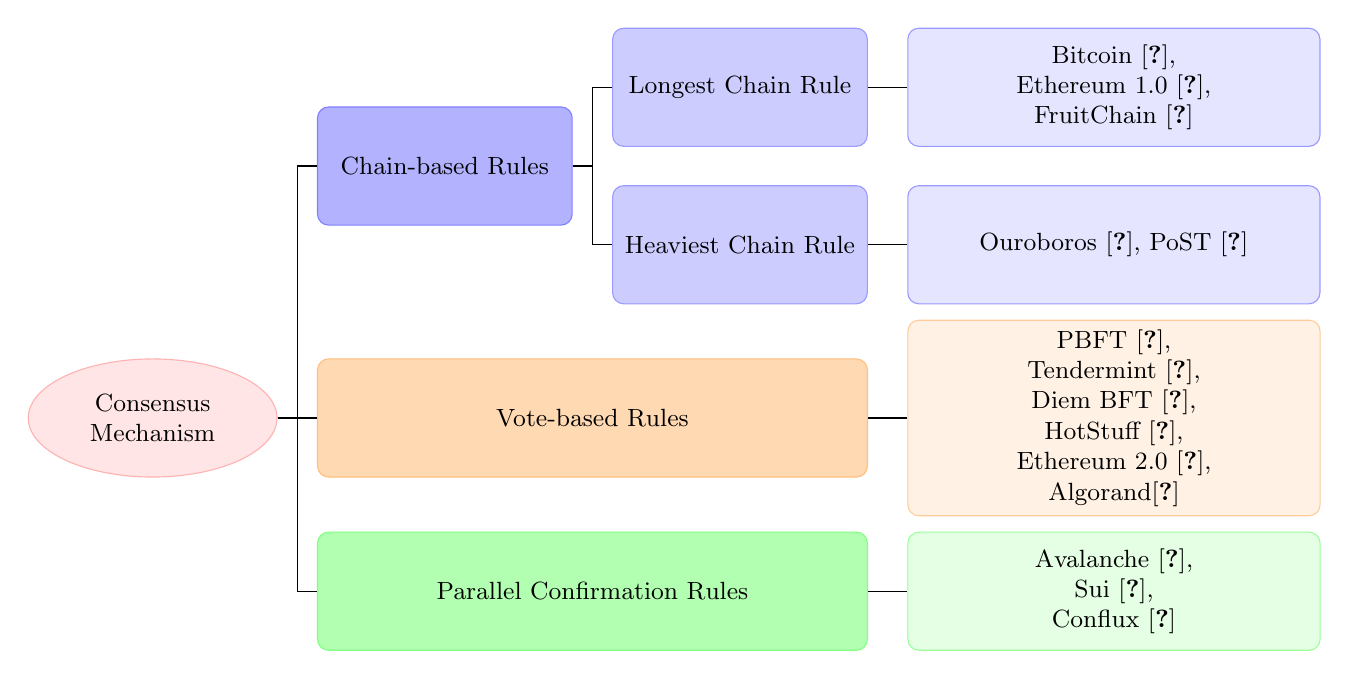
\begin{tikzpicture}[  
    node distance=0.5cm, % 节点之间的默认距离  
    every node/.style={align=center, font=\small, text centered, minimum height=1.5cm, rounded corners}, % 圆角矩形  
    every edge/.style={ultra thin, draw=black},  
]  

% 根节点  
\node[ellipse, draw=red!30, fill=red!10, text width=2cm] (root) {Consensus Mechanism};  

% 第一层节点(不同颜色)  
\node[rectangle, draw=blue!50, fill=blue!30, text width=3cm, right=of root, yshift=3.2cm] (chain) {Chain-based Rules};  
\node[rectangle, draw=orange!50, fill=orange!30, text width=6.75cm, right=of root] (vote) {Vote-based Rules};  
\node[rectangle, draw=green!50, fill=green!30, text width=6.75cm, right=of root, yshift=-2.2cm] (parallel) {Parallel Confirmation Rules};  

% 连接根节点到第一层节点  
\draw (root.east) -- ++(0.25,0) |- (chain.west);  
\draw (root.east) -- ++(0.25,0) |- (vote.west);  
\draw (root.east) -- ++(0.25,0) |- (parallel.west);  

% Chain-based Rules 的子节点(浅色版本)  
\node[rectangle, draw=blue!40, fill=blue!20, text width=3cm, right=of chain, yshift=1cm] (longest) {Longest Chain Rule};  
\node[rectangle, draw=blue!40, fill=blue!20, text width=3cm, right=of chain, yshift=-1cm] (heaviest) {Heaviest Chain Rule};  

% 连接 Chain-based Rules 到子节点  
\draw (chain.east) -- ++(0.25,0) |- (longest.west);  
\draw (chain.east) -- ++(0.25,0) |- (heaviest.west);  

% 最下面一层共识协议节点(浅色版本)  
\node[rectangle, draw=blue!40, fill=blue!10, text width=5cm, right=of longest] (bitcoin) {Bitcoin \cite{nakamoto2008bitcoin},\\ Ethereum 1.0 \cite{wood2014ethereum},\\ FruitChain \cite{pass2017fruitchains}};  
\node[rectangle, draw=blue!40, fill=blue!10, text width=5cm, right=of heaviest] (ouroboros) {Ouroboros \cite{kiayias2017ouroboros}, PoST \cite{moran2019simple}};  
\node[rectangle, draw=orange!40, fill=orange!10, text width=5cm, right=of vote] (pbft) {PBFT \cite{castro1999practical}, \\Tendermint \cite{buchman2016tendermint}, \\Diem BFT \cite{team2021diembft},\\ HotStuff \cite{yin2019hotstuff},\\ Ethereum 2.0 \cite{buterin2020combining},\\Algorand\cite{chen2019algorand}};  
\node[rectangle, draw=green!40, fill=green!10, text width=5cm, right=of parallel] (avalanche) {Avalanche \cite{rocket2019scalable}, \\ 
Sui \cite{blackshear2023sui}, \\
Conflux \cite{li2020decentralized}};  

% 连接最下面一层节点  
\draw (longest.east) -- ++(0.25,0) |- (bitcoin.west);  
\draw (heaviest.east) -- ++(0.25,0) |- (ouroboros.west);  
\draw (vote.east) -- ++(0.25,0) |- (pbft.west);  
\draw (parallel.east) -- ++(0.25,0) |- (avalanche.west);  
\end{tikzpicture}
\caption{Blockchain Consensus Protocol Classification}
\end{figure*}

%Consensus protocols are critical in blockchain systems as they ensure that all participants agree on the validity of transactions and the state of the blockchain. These protocols prevent unauthorized changes and secure the integrity of the distributed network by enabling all nodes to reach a common agreement. 
Blockchain consensus mechanisms can be classified based on their chain selection rules, including chain-based rules, vote-based rules, DAG-based rules.

\paragraph{Chain-based Consensus Rules.} 
Chain-based consensus rules rely on a linear blockchain structure, where blocks are linked in a chain, and the main chain is determined by the accumulated work or weight. 
The Longest Chain Rule, used in Proof-of-Work (PoW) systems like Bitcoin \cite{nakamoto2008bitcoin} and Ethereum 1.0 \cite{wood2014ethereum}, selects the chain with the most computational work. FruitChain \cite{pass2017fruitchains} extends the Longest Chain Rule by incorporating a dual-reward system, where miners earn rewards not only for block creation but also for broadcasting ``fruit'' structures, thus enhancing system security. 
Similarly, the Heaviest Chain Rule selects the chain with the greatest accumulated weight, typically based on stake, as seen in systems like Ouroboros \cite{kiayias2017ouroboros}. Additionally, Proof of Space and Time (PoST) \cite{moran2019simple} relies on the amount of storage and time invested to secure the chain, using a similar structure where the "heaviest" chain is the one that accumulates the most storage and time.

\paragraph{Vote-based Consensus Rules.} 
These consensus protocols involve nodes casting votes on the validity of transactions or blocks. 
In vote-based consensus systems, such as Practical Byzantine Fault Tolerance (PBFT) \cite{castro1999practical}, Tendermint \cite{buchman2016tendermint}, Algorand \cite{chen2019algorand} and HotStuff \cite{yin2019hotstuff}, a multi-phase voting process ensures that once a block is committed, it cannot be reverted, thus preventing forks. 
These protocols offer strong finality guarantees, with blocks being immediately finalized once they receive a sufficient number of votes.

\paragraph{Parallel Confirmation Rules.} Parallel confirmation rules deviate from traditional chain-based structures by allowing multiple branches to exist in parallel. 
In protocols like Avalanche \cite{rocket2019scalable}, Conflux \cite{li2020decentralized}, and Sui \cite{blackshear2023sui}, consensus is achieved probabilistically, with transactions validated concurrently across different branches. 
Since there is no main chain, consensus is reached without relying on a single-chain structure. 

It is also important to note that some consensus mechanisms may exhibit both primary and secondary attributes, blending features from different categories. 
For example, Ethereum 2.0 \cite{buterin2020combining} primarily relies on vote-based consensus (LMD-GHOST), while also incorporating the heaviest chain rule (via stake-weighted mechanisms) as a secondary feature.

\subsection{Design Components Across Different Consensus Protocols}

%The general MDP-based automated analysis framework for strategic mining focuses on identifying adversarial strategies targeting an incentive mechanism. 
%Constructing the environment and selecting an appropriate RL algorithm are key steps in this process. 
%The environment construction depends on the specific incentive mechanism and the underlying consensus algorithm. 
In this section, we outline the similarities and differences in environment construction for various consensus protocols, highlighting key design components such as \textit{state space}, \textit{action space}, and \textit{reward design}.

\paragraph{State Space.}
The state space must encode three critical components: (1) Action availability: features representing permissible actions in the current state, such as the fork status in Bitcoin (to track competing chains) \cite{sapirshtein2016optimal} or the match flag indicating active participation in protocols like LC-PoS \cite{sarenche2024deep}.
(2) Reward computation: features enabling reward calculation based on the canonical chain or subgraph. For example, in Bitcoin, this involves tracking the lengths of competing chains ($l_a, l_h$) to resolve forks \cite{nakamoto2008bitcoin}. For protocols with non-linear reward mechanisms (e.g., FruitChain’s "fruits" \cite{pass2017fruitchains,zhang2019lay} or Ethereum 2.0’s attestations \cite{zhang2024max}), additional metrics are required to compute relative rewards.
(3) State transition: The system state evolves through block generation, a discrete-time process with probability determined by mining power in PoW or stake in PoS. Transitions follow the consensus protocol’s stochastic rules and network assumptions, including idealized instant block propagation. During ties, honest nodes adopt adversarial blocks with a probability (rushing factor), modeling latency exploitation.


%As new blocks are generated, the system state transitions according to the consensus protocol's random rules and underlying network assumptions. Block generation is modeled as a discrete-time process, with the probability determined by mining power in PoW protocols or stake in PoS protocols. The network is assumed to propagate blocks instantly, and in the event of a tie, honest nodes follow the adversarial block with a probability known as the rushing factor.Accordingly, the state space must incorporate two key elements: i) the actions available in the current state, such as the fork status in Bitcoin \cite{sapirshtein2016optimal} and the match flag to indicate whether the action is active in LC-PoS protocol \cite{sarenche2024deep}; and ii) the ability to compute rewards based on specific states and actions. To calculate rewards, the state space should first involve the features that enable the identification of the canonical chain or subgraph, which in Bitcoin typically requires maintaining records such as the length of competing chains $l_a$ and $l_h$. Additionally, for rewards not solely based on block length, more detailed features need to be employed to compute relative rewards, such as the number of fruits in FruitChain \cite{pass2017fruitchains,zhang2019lay} or attestations in Ethereum 2.0 \cite{zhang2024max}.

\paragraph{Action Space.}
The design of the action space is closely tied to the adversarial model. 
For each consensus mechanism, different types of adversaries can be defined. 
For example, in the Bitcoin protocol, the action space is defined as {\textit{adopt, override, wait, match}}. 
Other attack strategies may involve actions outside this predefined space, such as the consideration of petty compliant miners in \cite{bar2023deep}. 
In the selfish proposing attack targeting the LC-PoS protocol \cite{sarenche2024deep}, the action space includes sub-actions to capture the `jump' strategy, allowing a selfish proposer to alter the parent block due to the ``nothing-at-stake'' property. 
In Ethereum 2.0, the action space may exclude the `match' action, as the rule for determining the canonical chain is based on the heaviest chain rather than the longest chain. 
This distinction removes the need to consider network propagation when competing chains have equal block lengths.

\paragraph{Reward Design.}
In reward design, previous approaches have primarily focused on relative rewards, defined as the attacker's rewards as a fraction of the total network rewards. 
These rewards are typically established on a per-unit basis, such as for blocks, as seen in earlier works. 
However, rewards can also be more intricately characterized, including transaction rewards \cite{bar2022werlman} and attestation rewards in Ethereum 2.0 \cite{zhang2024max}. 
The goal of the analysis is to identify a strategy $\pi: S \to \Delta(A)$ that maximizes the expected reward $R(s,a)$. 

%\paragraph{Objective Function.}The objective of analysis is to identify a strategy $\pi: S \to \Delta(A)$ that maximizes the expected reward $R(s,a)$. Accordingly, the \textit{state space} must incorporate two key elements: i) the actions available in the current state, such as the fork status in Bitcoin \cite{sapirshtein2016optimal} and the match flag to indicate whether the action is active in LC-PoS protocol \cite{sarenche2024deep}; and ii) the ability to compute rewards based on specific states and actions. To calculate rewards, the state space should first involve the features that enable the identification of the canonical chain or subgraph, which in Bitcoin typically requires maintaining records such as the length of competing chains $l_a$ and $l_h$. Additionally, for rewards not solely based on block length, more detailed features need to be employed to compute relative rewards, such as the number of fruits in FruitChain \cite{pass2017fruitchains,zhang2019lay} or attestations in Ethereum 2.0 \cite{zhang2024max}.

\subsection{Open Problems}
The evolution of blockchain technology and the digital economy has led to a significant shift from traditional longest-chain consensus mechanisms to alternative models. 
However, the economic security of these systems hinges on resolving critical open problems that remain inadequately addressed.
Moreover, the growing sophistication of miners in employing strategic mining techniques has introduced the risk of multi-agent strategic behaviors. These behaviors could destabilize the ecosystem, leading to economic inefficiencies or even systemic failures.
This section identifies important open problems in using RL for blockchain security analysis. 
Each problem highlights the need for advanced modeling techniques to address the complexities of modern blockchain systems.
%经济学安全
%每一组前面讲如果open problem做好了会有什么效果。

\paragraph{Open problem 1: How can extend strategic mining attack analysis to non-longest-chain consensus protocols?}

Existing research on strategic mining attacks has predominantly centered on longest-chain consensus protocols~\cite{eyal2014majority,sapirshtein2016optimal,sarenche2024deep}. 
To generalize this framework to alternative consensus mechanisms, three directions emerge:
\begin{itemize}
    \item \textbf{Weight-Based Protocols:} The state space must explicitly model weight accumulation dynamics. This requires incorporating weight-related parameters into the strategy space while preserving backward compatibility with existing analysis methods for longest-chain systems.
    \item \textbf{Parallel Proof-of-Work Protocols:}  The state space can be generalized to include additional features, such as topological order and uncle block rewards. These additions introduce multi-dimensional optimization challenges absent in linear chain protocols.
    \item \textbf{Vote-Based Consensus:} Participants attempt to minimize the costs associated with validating blocks and sending votes, which can result in coordination failures that undermine the validity of consensus protocols \cite{amoussou2020governing}. Furthermore, attackers can execute censorship attacks \cite{srivastava2024towards} by strategically excluding specific information from being incorporated into the final consensus.
\end{itemize}
Multiple tricks such as imposing artificial limits within the adversarial model \cite{sapirshtein2016optimal,zur2020efficient,hou2019squirrl} can help maintain a manageable state space size.
The application of the analysis framework to adversarial models targeting the aforementioned attacks still requires further exploration.

%For heaviest chain rule consensus, the state space can be modified to include weight-related information. 
%Similarly, for parallel proof-based consensus, the state space can be generalized to include additional features, such as topological order and uncle block rewards.
%The key challenge, however, is to incorporate the necessary features while avoiding excessive redundancy in the state space.
%Multiple tricks such as imposing artificial limits within the adversarial model \cite{sapirshtein2016optimal,zur2020efficient,hou2019squirrl} can help maintain a manageable state space size.

%For vote-based consensus, attackers exhibit distinct strategic behaviors.
% As mentioned above, strategic participants aim to maximize their expected rewards and deviate from the prescribed protocol only when such deviations offer higher expected payoffs.
% In vote-based consensus, participants attempt to minimize the costs associated with validating blocks and sending votes, which can result in coordination failures that undermine the validity or termination properties of consensus protocols \cite{amoussou2020governing}. Furthermore, attackers can execute censorship attacks \cite{srivastava2024towards} by strategically excluding specific information, such as transactions, from being incorporated into the final consensus.
% The application of the analysis framework to adversarial models targeting the aforementioned attacks still requires further exploration.

\paragraph{Open problem 2: How to develop more realistic MDP models for blockchain security?}

Current RL models for blockchain security rely on simplified assumptions, such as synchronized networks and fixed miner strategies \cite{zhang2019lay,sarenche2024deep}, to reduce complexity. However, in real-world environments, network conditions, miner strategies, and blockchain dynamics are highly unpredictable. For example, attackers may exploit network latency to conduct undetectable attacks, limiting the applicability of existing models \cite{bahrani2023undetectable}.

Future research should focus on relaxing these assumptions by incorporating dynamic, time-varying environments. RL models can account for unpredictable network delays, adaptive miner strategies, and changing blockchain dynamics. 
These uncertain conditions can be handle by using advanced RL algorithms, while ensuring robust security analysis under evolving threats.

\paragraph{Open problem 3: How can strategic mining be analyzed in multi-agent environments using RL?}
A key challenge is applying RL in multi-agent environments, where multiple miners or validators interact strategically to maximize rewards. In these environments, agents may compete, complicating the analysis of selfish mining attacks. 

\cite{marmolejo2019competing} use a Markov chain model to analyze multi-agent mining dynamics by simplifying the state space of selfish miners. This analysis restrict to semi-selfish mining, where miners only maintain private chains of length at most two. 
The Partially Observed Markov Game (POMG) extends MDP to multi-agent environments with partial information, allowing it to model strategic behaviors like selfish mining, such as SquirRL \cite{hou2019squirrl}. 
However, POMG has limitations, including assumptions about partial observability and challenges with scalability as the number of miners increases. Future research should focus on improving its scalability and refining agent interaction models to better capture the complexities and unpredictability of real-world blockchain dynamics.

\section{Conclusion}
\label{sec:conclusion}
This survey examines strategic mining in blockchain systems, with a focus on reinforcement learning as a tool for optimizing mining strategies.
%Our survey examines strategic mining in blockchain systems, emphasizing reinforcement learning as a tool for optimizing mining strategies. 
Traditional Markov Decision Process (MDP) approaches are useful for analyzing behaviors like selfish mining but face scalability challenges.
%Traditional Markov Decision Processes  approaches help analyze behaviors like selfish mining but struggle with scalability. 
Reinforcement learning (RL) provides adaptability in complex environments, enabling the identification of optimal strategies and security thresholds. 
This survey reviews previous studies that use MDPs and RL to analyze PoW and PoS consensus, and discusses the potential of these methods for analyzing other vote-based and parallel confirmation blockchains. 
%examines 
%RL's advantages over Markov Decision Processes (MDPs), especially in multi-agent settings, and proposes its potential to analyze vote-based and parallel confirmation blockchains.
%以前有了什么工作,将来要做什么。
%RL offers adaptability in complex environments, which can identify optimal strategies and security thresholds. The study highlights RL’s advantages over MDPs, particularly in multi-agent settings, and its potential in Proof-of-Stake blockchains. 
%Despite progress, challenges remain in modeling and multi-agent dynamics. 
Future research should focus on refining RL algorithms to improve blockchain security and efficiency, ultimately advancing decentralized systems.

%\appendix

%\section*{Ethical Statement}
%\section*{Acknowledgments}


%% The file named.bst is a bibliography style file for BibTeX 0.99c
\bibliographystyle{named}
\bibliography{ref}

\end{document}

